\documentclass[a4paper]{article}

\usepackage[swedish]{babel}
\usepackage[utf8]{inputenc}
\usepackage[intlimits]{amsmath}
\usepackage{hyperref}
\usepackage{underscore}
\usepackage{tikz}
\usepackage{tkz-euclide}
\usepackage{tikz-3dplot}
\usepackage{amsfonts}
\usepackage{mathtools}
\usepackage{enumitem}
\usepackage{blkarray}
\usepackage{xcolor}
\usepackage{amssymb}
\usepackage{siunitx}
\usepackage{fancyhdr}
\usepackage{lastpage}
\usepackage{xparse}
\usepackage{coffee4}
\usepackage{framed}
\usepackage{letltxmacro}
\usepackage{varioref}
\usepackage{pgfplots}

\usetkzobj{all}

\pgfplotsset{compat=1.10}
\usepgfplotslibrary{fillbetween}

\NewDocumentEnvironment{spmatrix}{ m }
  {\mathop\bgroup\begin{pmatrix}}
  {\end{pmatrix}\egroup_{\textstyle\mathstrut #1}}

\newcommand{\svar}[1]{\underline{\underline{#1}}}

\DeclarePairedDelimiter \abs{\lvert}{\rvert}
\DeclarePairedDelimiter \norm{\lVert}{\rVert}

\everymath{\displaystyle}

\let\oldsqrt\sqrt
\makeatletter
\let\oldr@@t\r@@t
\def\r@@t#1#2{
\setbox0=\hbox{$\oldr@@t#1{#2\,}$}\dimen0=\ht0
\advance\dimen0-0.2\ht0
\setbox2=\hbox{\vrule height\ht0 depth -\dimen0}
{\box0\lower0.4pt\box2}}
\LetLtxMacro{\oldsqrt}{\sqrt}
\renewcommand*{\sqrt}[2][\ ]{\oldsqrt[#1]{#2} }
\makeatother



\hypersetup{
	pdfauthor={Adnan Avdagic},
	pdftitle={TATA69 Föreläsningar},
	colorlinks}

\title{TATA69 Föreläsningar}
\author{Adnan Avdagic\\
	Linköpings Universitet\\
	\texttt{forelasningar@avdagic.net}}
\date{\today}

\begin{document}
\hypersetup{pageanchor=false}
\numberwithin{equation}{section}
\begin{titlepage}
\maketitle
\cofeAm{1}{1}{270}{100}{0}
\thispagestyle{empty}
\end{titlepage}


\cleardoublepage
\pagenumbering{gobble}
\tableofcontents
\cleardoublepage
\pagenumbering{arabic}




\newpage
\hypersetup{pageanchor=true}
\cleardoublepage
\setcounter{page}{1}
\setcounter{section}{1}
\pagestyle{fancy}
\fancyhf{}
\rhead{\textit{Adnan Avdagic}}
\lhead{Föreläsning \thesection}
\rfoot{\rightmark}
\lfoot{Sida \thepage}
\noindent
\section{Föreläsning II}
\subsection{Gränsvärden för flervarre}

\subsubsection{Exempel 1} \flushleft
\begin{equation} \label{eq:2.1}
	f(x,y) = \frac{\sin(x^4+y^2)}{x^4+y^2} \text{, ej definierad i origo}
\end{equation}

Vad händer då (x,y) närmar sig (0,0)?

$$\lim_{x,y \rightarrow 0,0} \frac{\sin(x^4+y^2)}{x^4+y^2}$$

//sätt $t= \displaystyle x^4+y^2$, ${t \rightarrow 0}$ då ${(x,y) \rightarrow (0,0)}$// \newline
då fås \(\displaystyle \lim_{t \rightarrow 0} \frac{\sin t}{t} = 1,\) (standard gränsvärde) \newline

\subsubsection{Exempel 2} \flushleft
\begin{equation} \label{eq:2.2}
	f(x,y) = \frac{x^3+xy}{x^2+y^2} \text{, ej definierad i origo}
\end{equation}

Gå mot origo via x-axeln (där $y=0$)
\[f(x,0) = \frac{x^3+0*x}{x^2+0^2} = \frac{x^3}{x^2} =  {x \rightarrow 0} \text{ då } {x \rightarrow 0}\]

Gå mot origo via y-axeln (där $x=0$)
\[f(0,y) = \frac{0^3+0*y}{0^2+y^2} = \frac{0}{y^2} =  {0 \rightarrow 0} \text{ då } {y \rightarrow 0}\]

Gå mot origo längs $y=x$
\[f(x,x) = \frac{x^3+x*x}{x^2+x^2} = {\frac{x+1}{2} \rightarrow \frac{1}{2}} \text{ då } {x \rightarrow 0}\]

Olika värden från olika riktningar \newline
Innanför varje liten cirkel kring origo har f värden nära 0 och nära $\frac{1}{2}$.
Vi säger därför att gränsvärde ej existerar. Se \vref{fig:2.1}

\begin{figure}[ht] 
\begin{tikzpicture}
   \tkzInit[xmax=5,ymax=5,xmin=-5,ymin=-5]
   \tkzAxeXY
   \draw[red,thick] (-5,0) -- (5,0);
   \draw[blue,thick] (0,-5) -- (0,5);
   \draw[green,thick] (-5,-2) -- (5,3);
   \node[above,red] at (-4,0) {\(f=x\)};
   \node[right,blue] at (0,5) {\(f=0\)};
   \node[left,green] at (3,3) {\(f=\frac{x+1}{2}\)};
   \tkzDefPoint(0,0){O}
   \tkzDefPoint(0.2,0.2){A}
   \tkzDrawCircle(O,A)
  \end{tikzpicture}
  \caption{Graf i 2D} \label{fig:2.1}
\end{figure}

\newpage
\subsubsection{Definition}

Funktionen \(\bar{f}\) av typ \(\mathbb{R}^n \rightarrow \mathbb{R}^m\) har gränsvärdet \(\bar{b} \in \mathbb{R}^m\) då 
\(\bar{x} \rightarrow \bar{a} \in \mathbb{R}^n\) om \(\forall \epsilon >0 \quad \exists \delta >0\) 
så att \(|\bar{f}(x)-\bar{b}|<\epsilon\) om \(0<|\bar{x}-\bar{a}|<\delta\) och \(\bar{x}\in D_f\). 
Skrivs 
\[
\lim_{\bar{x} \rightarrow \bar{a}} \bar{f}(\bar{x})=\bar{b}
\]

\newpage
\subsubsection{Exempel 3}
\begin{equation} \label{eq:2.3}
	f(x,y)=\frac{x^3}{x^2+y^2} \text{, ej definierad i origo}
\end{equation}

\[
\begin{split}
0 \leq \abs{f(x,y)} = \frac{\abs{x^3}}{x^2+y^2} = \abs{x}\frac{x^2}{x^2+y^2} \leq \abs{x} \rightarrow 0 \text{ då } (x,y) \rightarrow (0,0) \\
\Rightarrow f(x,y) \rightarrow (0,0) \text{ då } (x,y) \rightarrow (0,0)
\end{split}
\]

Vanliga räkneregler för gränsvärden (summa, produkt, instängning) gäller också för flervarregränsvärden
Undersökning/beräkning av gränsvärden

\begin{itemize}
\item Om test av värden längs olika riktningar eller olika kurvor ger olika resultat så saknas gränsvärde, se \eqref{eq:2.2}
\item Sådana test kan \underline{INTE} visa att gränsvärde existerar, andra metoder behövs, som \eqref{eq:2.1} eller \eqref{eq:2.3}, eller polära koordinater
\end{itemize}

\begin{figure}[ht] 
\begin{tikzpicture}
   \tkzInit[xmax=4,ymax=4,xmin=0,ymin=0]
   \tkzAxeXY
   \tkzDefPoint(3,3){P} \tkzDefPoint(0,0){O}
   \tkzDefPoint(3,0){a} \tkzDefPoint(0,3){b} \tkzDefPoint(1.5,0){c}
   \tkzDrawArc[color=red](O,c)(P)
   \tkzDrawPoints(P)
   \tkzDrawSegment[blue](O,P)
   \tkzDrawSegment[dashed](a,P)
   \tkzDrawSegment[dashed](b,P)
   \node[right,red] at (1.5,0.5) {$\varphi$};
   \node[above left,blue] at (1.5,1.5) {$\rho$};
   \node[above right] at (3,3) {(x,y)};
  \end{tikzpicture}
  \caption{Graf för polära koordinater} \label{fig:2.2}
\end{figure}

\[
	\def\arraystretch{1.1}
	\begin{blockarray}{r@{\;}l}
	\begin{block}{r@{\;}l\}}
		x & = \rho \cos(\varphi) \\[\jot]
		y & = \rho \sin(\varphi) \\[\jot]
	\end{block}
	\rho  & = \sqrt{x^2+y^2} \text{, } \rho > 0 \\ [\jot]
	\tan{\varphi} & = \frac{y}{x} \text{, } 0 \leq \varphi \leq 2\pi
	\end{blockarray}
\]
Viktigt för gränsvärden: \( (x,y) \rightarrow (0,0) \iff \rho \rightarrow 0 \)

\newpage

\paragraph{Exempel \eqref{eq:2.2} med polära koordinater}

\[
\begin{split}
\lim_{(x,y) \rightarrow 0} \frac{x^3+xy}{x^2+y^2} \overset{\,\mathrm{pol.koord}}{=} \lim_{\rho \rightarrow 0} \frac{\rho^3 \cos^3(\varphi) + \rho^2 \cos(\varphi) \sin(\varphi)}{\rho^2} = \\
=\lim_{\rho \rightarrow 0} (\overbrace{\rho \cos^3(\varphi)}^{\rightarrow 0}+\underbrace{\cos(\varphi) \sin(\varphi)}_\text{vinkelberoende}) \Rightarrow \text{gränsvärde existerar ej}
\end{split}
\]

\paragraph{Exempel \eqref{eq:2.3} med polära koordinater}

\[
	\lim_{(x,y) \rightarrow (0,0)} \frac{x^3}{x^2+y^2} \overset{\,\mathrm{pol.koord}}{=} \lim_{\rho \rightarrow 0} \frac{\rho^3\cos^3(\varphi)}{\rho^2} = 
	\lim_{\rho \rightarrow 0} \overbrace{\rho}^{\rightarrow 0}\underbrace{\cos^3(\varphi)}_\text{begränsad} = 0
\]

\subsection{Oändlighet i envarre och flervarre}
\subsubsection*{Envarre}
x kan gå mot $\pm\infty$
\subsubsection*{Flervarre}
bara en $\infty$ nämligen $\abs{\bar{x}} \rightarrow \infty$
\subsubsection*{2D polära}
$\abs{\bar{x}} \rightarrow \infty \iff \rho \rightarrow \infty$
\subsubsection{Definition}
\[
	\bar{f}(\bar{x}) \rightarrow \bar{b} \text{ då } \abs{\bar{x}} \rightarrow \infty \text{ om } \forall \epsilon > 0 \quad \exists \omega \text{ så att } \abs{\bar{f}(\bar{x}) - \bar{b}} < \epsilon \text{ om } \abs{\bar{x}} > \omega
\]

\newpage
\subsubsection{Exempel 4}

\begin{equation} \label{eq:2.4}
	\lim_{(x,y) \rightarrow \infty} \frac{y}{x^2+y^2} \overset{\,\mathrm{pol.koord}}{=} \lim_{\rho \rightarrow \infty} \frac{\rho \sin(\varphi)}{\rho^2} = 
	\lim_{\rho \rightarrow \infty} \overbrace{\frac{1}{\rho}}^{\rightarrow 0} \underbrace{\sin(\varphi)}_\text{Begränsad} = 0
\end{equation}

\paragraph{OBS!} 2-variabelfunktioner som uttryckta i polärakoordinater inte beror på $\varphi$ har rotationssymmetriska grafer kring z-axeln

\begin{figure}[ht]
\usetikzlibrary{3d}
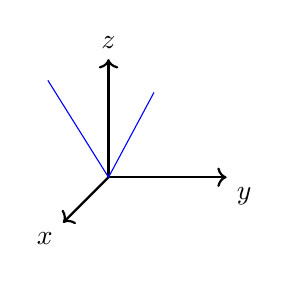
\begin{tikzpicture}
\draw[thick,->] (0,0,0) -- (0,0,1.5) node[anchor=north east]{$x$};
\draw[thick,->] (0,0,0) -- (1.5,0,0) node[anchor=north west]{$y$};
\draw[thick,->] (0,0,0) -- (0,1.5,0) node[anchor=south]{$z$};
\foreach \p in {1,...,360} {
	\draw[red] ({sin(45)*sin(\p)},{cos(45)},{sin(45)*cos(\p)}) -- ({sin(45)*sin(\p)},{cos(45)},{sin(45)*cos(\p)});
}
\draw[blue] (0,0,0) -- (0,2,2);
\draw[blue] (0,0,0) -- (0,0.5,-1.5);
\end{tikzpicture}
\caption{Exempel på rotationssymmetri} \label{fig:2.3}
\end{figure}

\(
z = \sqrt{x^2+y^2} = \rho
\)

\subsection{3-variabler mot origo}
\subsubsection{Exempel 5} 

\begin{equation} \label{eq:2.5}
	\lim_{(x,y,z) \rightarrow (0,0,0)} \frac{xyz}{x^2+y^2+2z^2} = \text{ ???}
\end{equation}

\[
	0 \leq \abs{\frac{xyz}{x^2+y^2+2z^2}} = \frac{\abs{x}\abs{y}\abs{z}}{x^2+y^2+2z^2} \leq \frac{\abs{x}\abs{y}\abs{z}}{x^2+y^2+z^2} \leq 
\]

\[
	// 
	\def\arraystretch{1.1}
	\begin{blockarray}{r@{\;}l}
	\abs{x} \leq \sqrt{x^2+y^2+z^2} \\ [\jot]
	\abs{y} \leq \sqrt{x^2+y^2+z^2} \\ [\jot]
	\abs{z} \leq \sqrt{x^2+y^2+z^2}
	\end{blockarray}
	//
\]

\[
\begin{split}
	\leq \frac{\sqrt{x^2+y^2+z^2}}{x^2+y^2+z^2} = \sqrt{x^2+y^2+z^2} \rightarrow 0 \text{ då } (x,y,z) \rightarrow (0,0,0) \\
	\Rightarrow \lim_{(x,y,z) \rightarrow (0,0,0)} \frac{xyz}{x^2+y^2+2z^2} = 0
\end{split}
\]

\newpage
\subsection{Rymdpolära koordinater}

\begin{figure}[ht]
\usetikzlibrary{3d}
\begin{tikzpicture}
\draw[thick,->] (0,0,0) -- (0,0,5) node[anchor=north east]{$x$};
\draw[thick,->] (0,0,0) -- (5,0,0) node[anchor=north west]{$y$};
\draw[thick,->] (0,0,0) -- (0,5,0) node[anchor=south]{$z$};
\draw[dashed]
	(0,4,0) --
	(4,4,4) coordinate (p) --
	(4,0,4) coordinate (q);
\draw[thick,red]
	(0,0,0) coordinate (o)-- (q);
\draw[dashed] 
	(0,0,4) coordinate (x) -- (q) -- (4,0,0);
\draw[thick,blue] (o) -- (p);
\draw[green] let
	\p0 = (o),
	\p1 = (0,0,2),
	\p2 = (2,0,2),
	\n1 = {atan2(\p1)},
    \n2 = {\n1 + 103},
    \n3 = {1cm},
    \n4 = {(\n1 + \n2) / 2}
  in (o) +(\n1:\n3) arc[radius = \n3, start angle = \n1, end angle = \n2];
\draw[purple] let
	\p0 = (o),
	\p1 = (0,0,2),
	\p2 = (2,0,2),
	\n1 = {atan2(2,0)},
    \n2 = {atan2(2,2)},
    \n3 = {1cm},
    \n4 = {(\n1 + \n2) / 2}
  in (o) +(\n1:\n3) arc[radius = \n3, start angle = \n1, end angle = \n2];
\node[fill,circle,inner sep=1.5pt,label={above right:$(x,y,z)$}] at (p) {};
\node[left,blue] at (2,2,2) {$r$};
\node[right,red] at (1,0,1) {$r\sin(\theta)$};
\node[above,green] at (1,0,2.5) {$\varphi$};
\node[above left,purple] at (0.7,1,0) {$\theta$};
\end{tikzpicture}
\caption{Rymdpolära koordinater} \label{fig:2.4}
\end{figure}

\[
\left\{\begin{array}{rcl}
	x & = r \sin(\theta) \cos(\varphi) \\
	y & = r \sin(\theta) \sin(\varphi) \\
	z & = r \cos(\theta) 
\end{array}\right.
\]
\[
\begin{split}
	r & = \sqrt{x^2+y^2+z^2} \text{, } r > 0 \\
	0 & \leq \theta \leq \pi \\
	r & \sin(\theta) = \rho
\end{split}
\]

För gränsvärden där \((x,y,z) \rightarrow (0,0,0) \iff r \rightarrow 0\)

\newpage
\paragraph{Exempel \eqref{eq:2.5} med rymdpolära koordinater}

\[
\begin{split}
	\lim_{(x,y,z) \rightarrow (0,0,0)} \frac{xyz}{x^2+y^2+2z^2} \overset{\,\mathrm{rymdpol.koord}}{=} \\
	= \lim_{r \rightarrow 0} \frac{r^3 \sin^2(\theta) \cos(\theta) \sin(\varphi) \cos(\varphi)}{r^2+r^2 \cos^2(\theta)} = \\
	= \lim_{r \rightarrow 0} \overbrace{r}^{\rightarrow 0} \underbrace{\frac{\sin^2(\theta) \cos(\theta) \sin(\varphi) \cos(\varphi)}{1+\cos^2(\theta)}}_\text{begränsad, nämnare \(\geq 1 \) ingen risk för /0}
\end{split}
\]

\subsubsection{Cylindriska koordinater}

Polära koordinater i (x,y) och vanliga i z

\[
\left\{\begin{array}{rcl}
	x & = r \cos(\varphi) \\
	y & = r \sin(\varphi) \\
	z & = z 
\end{array}\right.
\]






\newpage
\section{Föreläsning III}
\subsection{Partiella derivator}

\subsubsection{Exempel 1}

\begin{equation} \label{eq:3.1}
	f(x,y) = x^2y + x\sin(y)
\end{equation}

Hur förändras \(f\) om bara \(x\) varieras? Vi vill derivera \(f\) m.a.p \(x\) och hålla \(y\) konstant. Skrivs:

\[
	\underbrace{f^{\prime}_{x}(x,y) = \frac{\partial f}{\partial x}(x,y)}_{\text{båda skrivsätten används}} = 2xy+\sin(y)
\]

Motsvarande då bara \(y\) varieras

\[
	f^{\prime}_{y}(x,y) = \frac{\partial f}{\partial y}(x,y) = x^2 + x\cos(y)
\]

\subsubsection{Definition}

Partiella derivatan av \(f(x,y)\) m.a.p \(x\) i punkten \((x,y)\) är

\[
	f^{\prime}_{x}(x,y) = \lim_{h \rightarrow 0} \frac{f(x+h,y) - f(x,y)}{h}
\]

Om gränsvärde existerar! \newline

Motsvarande för y:

\[
	f^{\prime}_{y}(x,y) = \lim_{k \rightarrow 0} \frac{f(x,y+k) - f(x,y)}{k}
\]

\begin{figure}[ht] 
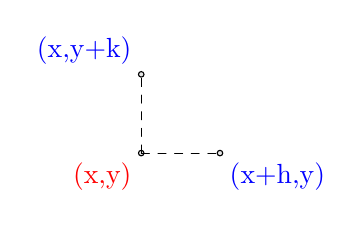
\begin{tikzpicture}
   \tkzInit[xmax=4,ymax=4,xmin=0,ymin=0]
   \tkzAxeXY
   \tkzDefPoint(2,2){a} \tkzDefPoint(3,2){b} \tkzDefPoint(2,3){c}
   \tkzDrawPoints(a,b,c)
   \tkzDrawSegment[dashed](a,b)
   \tkzDrawSegment[dashed](a,c)
   \node[below left,red] at (a) {(x,y)};
   \node[below right,blue] at (b) {(x+h,y)};
   \node[above left,blue] at (c) {(x,y+k)};
  \end{tikzpicture}
  \caption{Grafisk visning av hur f ändras i x- \& y-riktningen} \label{fig:3.1}
\end{figure}

\subsubsection{Exempel 2}

3 variabler

\begin{align*}
\begin{split}
	f(x,y,z) = x^3y^2z+z^2e^y \Rightarrow \\
	\Rightarrow \left\{\begin{array}{rcl}
		f_{x}^{\prime}(x,y,z) = & 3x^2y^2z \\
		f_{y}^{\prime}(x,y,z) = & 2x^3yz+z^2e^y \\
		f_{z}^{\prime}(x,y,z) = & x^3y^2+2ze^y
	\end{array}\right.
\end{split}
\end{align*}

\subsubsection{Andraderivator}

\[
\begin{split}
	f_{xx}^{\prime\prime} = \frac{\partial^2f}{\partial x^2} = \frac{\partial}{\partial x} \left(\frac{\partial f}{\partial x}\right) \\
	f_{xy}^{\prime\prime} = \frac{\partial^2f}{\partial y\partial x} = \frac{\partial}{\partial y} \left(\frac{\partial f}{\partial x}\right)
\end{split}
\]

\paragraph{Exempel \eqref{eq:3.1} andra derivator}

\[
	f_{xx}^{\prime\prime} = 2y
\]
\[
\left.\begin{array}{rcl}
	f_{xy}^{\prime\prime} = 2x + \cos(y) \\
	f_{yx}^{\prime\prime} = 2x + \cos(y)\\
\end{array}\right\}\text{lika, ingen slump}
\]
\[
	f_{yy}^{\prime\prime} = -x\sin(y)
\]

Skriv \(f\in C^r\) om \(f\):s alla \(r\):te-derivator är kontinuerlig.

\subsubsection{Sats}

\[
	f \in C^2 \Rightarrow f_{xy}^{\prime\prime} = f_{yx}^{\prime\prime}
\]

motsvarande för \(\geq 3\) varianter \newline

\(f(x,y)\) har 4 andraderivator varav 3 olika \\
\(f(x,y,z)\) har 9 andraderivator varav 6 olika

\newpage

\subsubsection{Exempel 3}

Bestäm alla \(f(x,y,z)\) som uppfyller

\begin{equation}
\begin{split}
	f_{x}^{\prime} = p(x,y,z) = 3x^2yz \quad (1) \\
	f_{y}^{\prime} = q(x,y,z) = x^3z + 2ye^z \quad (2) \\
	f_{z}^{\prime} = r(x,y,z) = x^3y + y^2e^z \quad (3) 
\end{split}
\end{equation}

\underline{Systematisk lösning}

\[
\begin{split}
	(1) \Rightarrow f(x,y,z) = x^3yz+\overbrace{\underbrace{g(y,z)}_{\text{2-variabel} f}}^{\text{godtycklig}} \\
	\underline{\text{Derivera detta m.a.p } y} \\
	\Rightarrow x^3z+g_{y}^{\prime}(y,z) = x^3z+2ye^z \Rightarrow \\
	\Rightarrow g_{y}^{\prime}(y,z) = 2ye^z \Rightarrow \\
	\Rightarrow g(y,z) = y^2e^z + \overbrace{\underbrace{h(z)}_{\text{envarre }f}}^{\text{godtycklig}} \Rightarrow \\
	\Rightarrow f(x,y,z) = x^3yz+y^2e^z+h(z) \\
	\underline{\text{Derivera detta m.a.p } z} \\
	\Rightarrow x^3y+y^2e^z+h^{\prime}(z) = x^3y+y^2e^z \Rightarrow \\									  	
	\Rightarrow h^{\prime}(z) = 0 \Rightarrow h(z) = C \Rightarrow
\end{split}
\]

\[
	\Rightarrow \text{Svar: } f(x,y,z) = x^3yz+y^2e^z+C \text{ ,\(C\) är en godtycklig konstant}
\]

\centerline{Man kan visa att systemet (1) - (3) är lösbart}
\[
	\iff
\]
\[
\begin{split}
	p_{y}^{\prime} = q_{x}^{\prime} \\
	p_{z}^{\prime} = r_{x}^{\prime} \\
	q_{z}^{\prime} = r_{y}^{\prime} 
\end{split}
\]

\subsubsection{Exempel 4}

\[
\begin{split}
	f_{x}^{\prime} = xy \\
	f_{y}^{\prime} = x^2 \\
	\text{olösbart ty} \\
	f_{xy}^{\prime\prime} = x \neq f_{yx}^{\prime\prime} = 2x
\end{split}
\]

\subsection{Differentierbarhet}
\subsubsection*{Envarre}

Om \(f_{a}^{\prime} = \lim_{h \rightarrow 0} \frac{f(a+h) - f(a)}{h} \quad \exists\) (dvs \(f\) deriverbar i \(a\)) så finns talet \(f_{a}^{\prime} = A\) sådant att \(\frac{f(a+h) - f(a)}{h}-A = 
\frac{1}{h}(f(a+h)-f(a)-Ah) = \rho(h) \rightarrow 0\) \newline \newline
Vi vet att \(f \in C^1 \Rightarrow f\) deriverbar \(\Rightarrow f\) kontinuerlig 

\subsubsection*{Flervarre}
\subsubsection{Definition}

\(f(x,y)\) är \underline{differentierbar} i \((a,b)\) om \(\exists\) tal \(A,B\) så att

\[
	\frac{1}{\sqrt{h^2+k^2}} (f(a+h,b+k) - f(a,b) - Ah - Bk) = \rho(h,k) \rightarrow 0 \text{ då } (h,k) \rightarrow (0,0)
\]

så deriverbar = differentierbar för envarre
För \(\geq\) 2 variabler gäller

\subsubsection{Sats}

\[
	f \in C^1 \overset{(1)}{\Rightarrow} f \text{ differentierbar} \left\{\begin{array}{rcl}
	\overset{(2)}{\Rightarrow} f \text{ partiellt deriverbar} \overset{(4)}{\nRightarrow} f \text{ kontinuerlig} \\
	\overset{(3)}{\Rightarrow} f \text{ kontinuerlig} \overset{(5)}{\nRightarrow} f \text{ partiellt deriverbar}
	\end{array}\right.
\]

\paragraph{Förklaring av pilar}
\begin{enumerate}
	\item s.56-57 i boken
	\item \(
				f_{x}^{\prime}(a,b) = \lim_{h \rightarrow 0} \frac{f(a+h,b) - f(a,b)}{h} \overset{f \text{ diff.bar med }k=0}{=} \lim_{h \rightarrow 0} \frac{Ah + B*0 + \sqrt{h^2 + 0^2}\rho(h,0)}{h} = 
				\lim_{h \rightarrow 0} A  + \underbrace{\frac{\sqrt{h^2}}{h}}_{\pm \text{ 1 begränsad}} \underbrace{\frac{\rho(h,0)}{h}}_{\rightarrow 0} = A \quad \exists
			\)
	\item \(
				f(a+h,b+k) = f(a,b) + \underbrace{Ah}_{\rightarrow 0} + \underbrace{Bk}_{\rightarrow 0} + \underbrace{\sqrt{h^2 + k^2}}_{\rightarrow 0}\underbrace{\rho(h,k)}_{\rightarrow 0} \rightarrow f(a,b) 
				\text{ då } (h,k) \rightarrow (0,0) \Rightarrow f \text{ kontinuerlig}
			\)
	\item Motexempel finns i boken s.51
	\item Motexempel \(f(x,y) = \abs{x}\) i \((0,0)\), kontinuerlig men \(f_{x}^{\prime}(x,y) \quad \nexists\)
\end{enumerate}

\newpage

\subsubsection{Linjär avbildning}

Den linjära avbildningen \(df_{(a,b)}\) av typ \(\mathbb{R}^2 \rightarrow \mathbb{R}\), som definieras av \(df_{(a,b)}(h,k) = Ah + Bk = 
f_{x}^{\prime}(a,b)h + f_{y}^{\prime}(a,b)k\), kallas \underline{differentialen} av \(f\) i (a,b) \\
ofta skrivs variablerna \(h=\,\mathrm{d}x\) \& \(k=\,\mathrm{d}y\) så \(df_{(a,b)}(\,\mathrm{d}x,\,\mathrm{d}y) = f_{x}^{\prime}(a,b)\,\mathrm{d}x + f_{y}^{\prime}(a,b)\,\mathrm{d}y\) eller kort \(df = f_{x}^{\prime}\,\mathrm{d}x + f_{y}^{\prime}\,\mathrm{d}y\)

\paragraph{Exempel \eqref{eq:3.1} omskrivet}

\[
	f(x,y) = x^2y + x\sin(y) \Rightarrow df = (2xy+\sin(y))\,\mathrm{d}x + (x^2+x\cos(y))\,\mathrm{d}y
\]

\subsubsection*{Feluppskattning med \(df\)}

Om \(\overline{\Delta x} = (\Delta x_{1},...,\Delta x_{n}) \in \mathbb{R}^n\) och \(f\) är differentierbar fås 
\(f(\overline{x} + \overline{\Delta x}) - f(\overline{x}) = 
f_{x_{1}}^{\prime}\Delta x_{1} + ... + f_{x_{n}}^{\prime}\Delta x_{n} + \underbrace{\rho(\Delta x_{1},...,\Delta x_{n})\sqrt{(\Delta x_{1})^2 + ... + (\Delta x_{n})^2}}_{\text{Restterm}} \approx df(\overline{\Delta x})\) 

\subsubsection{Exempel 5}

Bestäm rörelseenergin och uppskatta felet för massan \(m = 1.0 \pm 0.1\si{\kilogram}\) med hastigheten \(v = 4.0 \pm 0.2\si{\metre\per\second}\). \newline
Formel för rörelseenergi: \(E = \frac{mv^2}{2} \si{\joule}\) \newline
Utan fel: \(E = \frac{1*1.4^2}{2} = 8.0 \si{\joule}\) \newline
Fel: 
\[
\begin{split}
	\Delta E = E(m + \Delta m, v + \Delta v) - E(m,v) \approx dE(\Delta m,\Delta v) = \\
	= \frac{\partial E}{\partial m} \Delta m + \frac{\partial E}{\partial v} \Delta v = \underbrace{\frac{v^2}{2}}_{\frac{4^2}{2}} \Delta m + \underbrace{mv}_{1*4} \Delta v = 8\Delta m + 4\Delta v \\
	\Rightarrow \text{ maxfel } \leq 8\abs{\Delta m} + 4\abs{\Delta v} = 8*0.1 + 4*0.2 = 1.6 \si{\joule} \Rightarrow E = 8.0 \pm 1.6 \si{\joule}
\end{split}
\]





\newpage
\section{Föreläsning IV}
\subsection{Kedjeregeln}

\subsubsection*{Envarre}

\underline{Exempel} \[\frac{d}{\,\mathrm{d}x} e^{x^2} = e^{x^2}2x\]

\underline{Allmänt} \[f(g(x)) = \underbrace{f^{\prime}(g(x))}_{\text{yttre}} \underbrace{g^{\prime}(x)}_{\text{inre}} \]

\paragraph{Generalisering till flervarre}

\[
	\underbrace{f(g(x))}_{\text{envarre}} \Rightarrow \left\{\begin{array}{rcl}
	\overset{(1)}{\Rightarrow} f(g(\bar{x})) \\
	\overset{(2)}{\Rightarrow} f(\bar{g}(x))
	\end{array}\right\}
	\overset{(3)}{\Rightarrow} f(\bar{g}(\bar{x})) \Rightarrow \bar{f}(\bar{g}(\bar{x}))
\]

\paragraph{Förklaring av pilar}
\begin{enumerate}
	\item \subsubsection*{Exempel 1}
	\[
	\begin{split}
		\frac{\partial}{\partial x} e^{x^2 y} = e^{x^2 y}*\underbrace{2xy}_{\text{inre m.a.p }x} \\
		\frac{\partial}{\partial y} e^{x^2 y} = e^{x^2 y}*\underbrace{x^2}_{\text{inre m.a.p }y}
	\end{split}
	\]
	\subsubsection*{Allmänt}
	\[
		\left\{\begin{array}{rcl}
		\frac{\partial}{\partial x} f(g(x,y)) = f^{\prime}(g(x,y))g_{x}^{\prime}(x,y) \\
		\frac{\partial}{\partial y} f(g(x,y)) = f^{\prime}(g(x,y))g_{y}^{\prime}(x,y)
		\end{array}\right.
	\]
	Motsvarande för \(\geq\) 3 variabler
	\subsubsection*{Exempel 2}
	Visa att \(xh_{x}^{\prime} - 2yh_{y}^{\prime} = 0 \quad \forall\) 2 variabel funktioner \(h(x,y)\) 
	på formen \(h(x,y) = f(x^2y)\) där \(f\) är en envariabelfunktion. Lösning:
	\[
		xh_{x}^{\prime} - 2yh_{y}^{\prime} = xf^{\prime}(x^2y)2xy - 2yf^{\prime}(x^2y)x^2 = 0 \quad \forall f
	\]
	
	\newpage
	\item
	\[
	\begin{split}
		\frac{d}{\,\mathrm{d}x}(f(\bar{g}(x))) = \frac{d}{\,\mathrm{d}x}(f(g_{1}(x),g_{2}(x))) \overset{\text{def av }\frac{d}{\,\mathrm{d}x}}{=} \\
		= \lim_{l \rightarrow 0} \frac{f(\overbrace{g_{1}(x+l)}^{s+h},\overbrace{g_{2}(x+l)}^{t+k}) - 
		f(\overbrace{g_{1}(x)}^{s},\overbrace{g_{2}(x)}^{t})}{l} \underset{\text{diff.bar}}{=} \\
		= \lim_{l \rightarrow 0} \frac{f_{s}^{\prime}(s,t)h+f_{t}^{\prime}(s,t)k+\sqrt{h^2+k^2}\rho(h,k)}{l} = 
	\end{split}
	\]
	\[
		= \left/ \begin{array}{rcl}
			h=g_{1}(x+l)-g_{1}(x) \rightarrow 0 \text{ då } l \rightarrow 0 \text{ om \(g_{1}\) är kontinuerlig} \\
			k=g_{2}(x+l)-g_{1}(x) \rightarrow 0 \text{ då } l \rightarrow 0 \text{ om \(g_{2}\) är kontinuerlig}
		\end{array}\right/ =
	\]
	\[
		= \lim_{l \rightarrow 0} \left(
		 f_{s}^{\prime}(s,t)\overbrace{\frac{g_{1}(x+l)-g_{1}(x)}{l}}^{\rightarrow g_{1}^{\prime}(x)}+
		 f_{t}^{\prime}(s,t)\overbrace{\frac{g_{2}(x+l)-g_{2}(x)}{l}}^{\rightarrow g_{2}^{\prime}(x)}\pm
		 \sqrt{\underbrace{\left(\frac{h}{l}\right)^2+\left(\frac{k}{l}\right)^2}
		 _{\rightarrow (g_{1}^{\prime}(x))^2+(g_{2}^{\prime}(x))^2 \text{ begränsad}}}
		 \overbrace{\rho(h,k)}^{\rightarrow 0} 
		\right) =
	\]
	\[
	\begin{split}
		= f_{s}^{\prime}(s,t)g_{1}^{\prime}(x) + f_{t}^{\prime}(s,t)g_{2}^{\prime}(x) \\
		\text{eller } \frac{df}{\,\mathrm{d}x} = f_{s}^{\prime}s_{x}^{\prime} + f_{t}^{\prime}t_{x}^{\prime}
	\end{split}
	\]
	\item \subsubsection*{Fås av 1 \& 2}
	\[
	\begin{split}
		\frac{\partial}{\partial x}f(\overbrace{g_{1}(x,y)}^{s},\overbrace{g_{2}(x,y)}^{t}) = f_{s}^{\prime}s_{x}^{\prime} +
		f_{t}^{\prime}t_{x}^{\prime} \\
		\frac{\partial}{\partial y}f(g_{1}(x,y),g_{2}(x,y)) = f_{s}^{\prime}s_{y}^{\prime} + f_{t}^{\prime}t_{y}^{\prime}
	\end{split}
	\]
	\subsubsection*{Matrisform}
	\[
	\underbrace{\begin{pmatrix} f_{x}^{\prime} & f_{y}^{\prime} \end{pmatrix}}_{\text{derivator av }f(x,y)} =
	\underbrace{\begin{pmatrix} f_{s}^{\prime} & f_{t}^{\prime} \end{pmatrix}}_{\text{derivator av }f(s,t)}
	\begin{pmatrix} s_{x}^{\prime} & s_{y}^{\prime} \\ t_{x}^{\prime} & t_{y}^{\prime} \end{pmatrix}
	\]
	Motsvarande för \(\geq\) 3 variabler
\end{enumerate}

\newpage
\subsubsection{Exempel 1} Lös den partiella differentialekvationen
\begin{equation} \label{eq:4.1}
	f_{x}^{\prime} - f_{y}^{\prime} = y-x
\end{equation}
med bivillkoret 
\begin{equation}\label{eq:4.2}
	f(x,0) = x^2
\end{equation}
\[
\begin{split}
	\text{Ledning: inför nya variabler } \left\{\begin{array}{rcl}
	s = x+y \\ t = xy
	\end{array}\right.
\end{split}
\]
\[
\begin{split}
	\text{Kedjeregeln } \left\{\begin{array}{rcl}
		f_{s}^{\prime}s_{x}^{\prime} + f_{t}^{\prime}t_{x}^{\prime} = 
		f_{s}^{\prime}*1 + f_{t}^{\prime}y \\
		f_{s}^{\prime}s_{y}^{\prime} + f_{t}^{\prime}t_{y}^{\prime} =
		f_{s}^{\prime}*1 + f_{t}^{\prime}x
	\end{array}\right.
	\text{sätt in i \eqref{eq:4.1}} \\
	\Rightarrow (f_{s}^{\prime}+f_{t}^{\prime}y) - (f_{s}^{\prime}+f_{t}^{\prime}x) = y-x
	\Rightarrow f_{t}^{\prime}*(y-x) = y-x \text{, ska gälla alla } (x,y) \\
	\Rightarrow f_{t}^{\prime} = 1 \Rightarrow f_{t} = t + \underbrace{g(s)}_{godtycklig}
	\Rightarrow \underline{f(x,y) = xy + g(x,y)} \text{ [alla lösningar på \eqref{eq:4.1}]}
\end{split}
\]
Bivillkoret \eqref{eq:4.2} ger oss \(f(x,0) = x * 0 + g(x) = x^2 \Rightarrow g(x+0) = x^2 \Rightarrow\)
Lösningen blir \(f(x,y) = xy + (x+y)^2\)

\subsubsection{Linjärt variabelbyte}

\[
\left\{\begin{array}{rcl}
	s = ax + by \\
	t = cx + \,\mathrm{d}y
\end{array}\right.
\Rightarrow \begin{spmatrix}{X_{\underbar{f}}}s \\ t\end{spmatrix} =
\begin{spmatrix}{T^{-1}}a & b \\ c & d\end{spmatrix}
\begin{spmatrix}{X_{\underbar{e}}}x \\ y\end{spmatrix}
\]

Matris för kedjeregeln

\[
\begin{pmatrix} s_{x}^{\prime} & s_{y}^{\prime} \\ t_{x}^{\prime} & t_{y}^{\prime} \end{pmatrix} =
\begin{pmatrix}a & b \\ c & d\end{pmatrix} = T^{-1} \text{ !}
\]

\subsubsection{Byte till polära koordinater}

\[
\left\{\begin{array}{rcl}
	x = \rho\cos(\varphi) \\
	t = \rho\sin(\varphi)
\end{array}\right.
\text{Enklast med \(\rho\) \& \(\varphi\) derivator i vänsterled i kedjeregeln}
\]

\[
\left\{\begin{array}{rcl}
	f_{\rho}^{\prime} = f_{x}^{\prime}x_{\rho}^{\prime} + f_{y}^{\prime}y_{\rho}^{\prime} =
	f_{x}^{\prime}\cos(\varphi) + f_{y}^{\prime}\sin(\varphi) \\
	f_{\varphi}^{\prime} = f_{x}^{\prime}x_{\varphi}^{\prime} + f_{y}^{\prime}y_{\varphi}^{\prime} =
	f_{x}^{\prime}(-\rho\sin(\varphi)) + f_{y}^{\prime}\rho\cos(\varphi)
\end{array}\right.
\]

Matrisform

\[
	\begin{pmatrix}f_{\rho}^{\prime} & f_{\varphi}^{\prime}\end{pmatrix} =
	\begin{pmatrix}f_{x}^{\prime} & f_{y}^{\prime}\end{pmatrix}
	\begin{pmatrix}x_{\rho}^{\prime} & x_{\varphi}^{\prime} \\
	y_{\rho}^{\prime} & y_{\varphi}^{\prime}\end{pmatrix} =
	\begin{pmatrix}f_{x}^{\prime} & f_{y}^{\prime}\end{pmatrix}
	\begin{pmatrix}\cos(\varphi) & \sin(\varphi) \\
	-\rho\sin(\varphi) & \rho\cos(\varphi)\end{pmatrix}
\]

\newpage

\subsubsection{Exempel 2} \label{eq:4.3}
Bestäm alla \(f(x,y)\) som uppfyller
\begin{equation}
	xf_{xy}^{\prime\prime} - yf_{yy}^{\prime\prime} - f_{y}^{\prime} = 0
\end{equation}

\[
\text{Ledning: inför }
\left\{\begin{array}{rcl}
	u = x \\
	v = xy
\end{array}\right.
\]

Översätt ekvationen till u \& v. Kedjeregeln
\[
\left\{\begin{array}{rcl}
	f_{x}^{\prime} = f_{u}^{\prime}u_{x}^{\prime} + f_{v}^{\prime}v_{x}^{\prime} = f_{u}^{\prime} + yf_{v}^{\prime} \\
	f_{y}^{\prime} = f_{u}^{\prime}u_{y}^{\prime} + f_{v}^{\prime}v_{y}^{\prime} = xf_{v}^{\prime} 
\end{array}\right.
\]

Operator skrivsätt
\[
\left\{\begin{array}{rcl}
	\frac{\partial}{\partial x} = \frac{\partial}{\partial u} + y\frac{\partial}{\partial v}\\
	\frac{\partial}{\partial y} = x\frac{\partial}{\partial v}
\end{array}\right.
\left\{\begin{array}{rcl}
	(\text{ })_{x}^{\prime} = (\text{ })_{u}^{\prime} + (\text{ })_{v}^{\prime} \\
	(\text{ })_{y}^{\prime} = x(\text{ })_{v}^{\prime}
\end{array}\right.
\]
\[
	f_{yy}^{\prime\prime} = (f_{y}^{\prime})_{y}^{\prime} = (xf_{v}^{\prime})_{y}^{\prime} = x(f_{v}^{\prime})_{y}^{\prime} = x * x(f_{v}^{\prime})_{v}^{\prime} = x^2 f_{vv}^{\prime\prime}
\]
\[
	f_{xy}^{\prime\prime} = (f_{x}^{\prime})_{y}^{\prime} = (f_{u}^{\prime} + yf_{v}^{\prime})_{y}^{\prime} =
	(f_{u}^{\prime})_{y}^{\prime} + f_{v}^{\prime} + y(f_{v}^{\prime})_{y}^{\prime} =
	xf_{uv}^{\prime\prime} + f_{v}^{\prime} + yxf_{vv}^{\prime\prime}
\]

Sätt in i \eqref{eq:4.2} \(\Rightarrow\)

\[
\begin{split}
	x(xf_{uv}^{\prime\prime}+f_{v}^{\prime}+yxf_{vv}^{\prime\prime}) - y(x^2f_{vv}^{\prime\prime}) - xf_{v}^{\prime} = 0 \\
	x^2 f_{uv}^{\prime\prime}+xf_{v}^{\prime}+yx^2f_{vv}^{\prime\prime} - yx^2f_{vv}^{\prime\prime} - xf_{v}^{\prime} = 0
\end{split}
\]
\[
\begin{split}
	\Rightarrow x^2f_{uv}'' = 0, \quad \forall (x,y) 
	\Rightarrow f_{uv}'' = 0 \iff (f_{u}')_{v}' \\
	\Rightarrow f_{u}^{\prime} = g(u) \text{ , godtycklig funktion }g(u) \\
	\Rightarrow f = G(u) + h(v) \text{ , godtycklig funktion }h(v)
\end{split}
\]
\[
	\text{\underline{Svar:} } f(x,y) = G(x) + h(xy) \text{ , }g=G^{\prime}\text{  }g\text{\&}h\text{ godtyckliga funktioner}
\]







\newpage
\section{Föreläsning V}

\subsection{Gradienter}

\subsubsection{Definition}

\underline{Gradienten} av \(f(x,y)\) är \underline{vektorn} \(\nabla f =\) grad \(f = (f'_{x},f'_{y})\) \newline
För \(g(x,y,z)\) är \(\nabla g = (g'_{x},g'_{y},g'_{z})\) och motsvarande för \(\geq\) 4 variabler \newline

\underline{Hessianen} av \(f(x,y)\) resp \(g(x,y,z)\) är \underline{matrisen} 
\[Hf=
\begin{pmatrix}
f''_{xx} && f''_{xy} \\
f''_{yx} && f''_{yy}
\end{pmatrix}\] 
\[\text{resp } Hg = 
\begin{pmatrix}
g''_{xx} && g''_{xy} && g''_{xz} \\
g''_{yx} && g''_{yy} && g''_{yz} \\
g''_{zx} && g''_{zy} && g''_{zz}
\end{pmatrix}\]

symmetriska om \(f,g \in C^2\), \newline mer om \(H\) i samband med max/min-problem. \vref{sec:Hessian}

\subsubsection{Hur tolkar man gradienter i 2D \& 3D?}

\subsubsection*{Kurvor i 2D}

Tangenter och normaler (allmänt)

Tangentvektor \(\bar{T} = (v_1,v_2)\) \newline
Normalvektor \(\bar{T} = k(v_2,-v_1)\) ty ger \newline

\[\bar{T} \bullet \bar{N} = v_1kv_2 - v_2kv_1 = 0 \Rightarrow \text{ortogonala}\]

Ekvivalent för tangentlinje i \((x,y)\) är på tangenten \(\iff\) \newline

\[\underbrace{(x-a,y-b)}_{\text{Parallell med }\bar{T}} \bullet \bar{N} = 0 \iff v_2x - v_1y = \underbrace{v_2a - v_1b}_{Konstant}\]

\[
	\text{Parameterform} 
	\left\{\begin{array}{rcl}
		x=a+tv_2 \\
		y=b+tv_2
	\end{array}\right.
	\text{ , } t \in \mathbb{R} \text{ parameter}
\]

Ekvation för normallinjen: \((x,y)\) är på normalen \(\iff\)
\[
	\underbrace{(x-a,y-b)}_{\text{Parallell med }\bar{N}} \times (v_1,v_2) = 0 \iff v_1x + v_2y = \underbrace{v_1a + v_2b}_{Konstant}
\]

\[
	\text{Parameterform} 
	\left\{\begin{array}{rcl}
		x=a+tv_1 \\
		y=b-tv_2
	\end{array}\right.
	\text{ , } t \in \mathbb{R}
\]

\newpage
\begin{enumerate}
\item Kurvor på parameterform
\subsubsection*{Ex}
\[
	\left\{\begin{array}{rcl}
		x=1-t \\
		y=2+t
	\end{array}\right.
	\iff (x,y) = (1,2) + t(-1,1) \quad \text{[rät linje]}
\]

\subsubsection*{Ex}
\[\bar{r}(t) = \Big(x(t),y(t)\Big) = \Big(\cos{t}, \sin{t}\Big) \quad \text{[enhetscirkeln]}\]
\[\text{Två punkter på kurvan } \bar{r}(t) \quad \& \quad \bar{r}(t+\Delta t)\]
\[\begin{split}
	\text{Låt } \Delta t \rightarrow 0 \Rightarrow \bar{T}(t) = r'(t) = 
	\lim_{\Delta t \rightarrow 0} \frac{\bar{r}(t+\Delta t) - \bar{r}}{\Delta t} = \Big(x'(t),y'(t)\Big) \\
	= \text{ ger tangentvektorn till kurvan, exempelvis har enhetscirkeln } \\
\end{split}\]
\[\bar{T}(t) = \Big(x'(t),y'(t)\Big) = \Big( -\sin{t},\cos{t} \Big)\]

\item Nivåkurvor \(f(x,y) = C\)
\paragraph{}
Om \(f(x,y) = C\) parametriseras med t som \(\Big(x(t),y(t)\Big)\) ger kedjeregeln 
\[
	0 = \frac{d}{dt} \overbrace{f\Big(x(t),y(t)\Big)}^{\text{konstant = C}} = f'_xx'(t)+f'_yy'(t) =
	\underbrace{\Big(f'_x,f'_y\Big)}_{\nabla f} \bullet \underbrace{\Big(x'(t),y'(t)\Big)}_{\bar{T}}
\]
\[\Rightarrow \nabla f \text{ är normalvektor till nivåkurvan}\] 

\subsubsection*{Ex}
Enhetscirkeln \(\Big[f(x,y)=x^2+y^2=1\Big]\) har \(\nabla f = \Big(2x,2y\Big) = 2\Big(x,y\Big)\)

\item
\subsubsection*{Grafer}

\(y=h(x)\) kan föras på 
\begin{itemize}
\item parameterform: \(t=x\) ger \(\Big(x,y\Big) = \Big(t,h(t)\Big) \) 
\(\Rightarrow \bar{T} = \Big(x',y'\Big) = \Big(t,h(t)\Big)\)

\item nivåkurveform: sätt \(f(x,y) = y-h(x) = 0\) \newline
\(\Rightarrow \bar{N} = \nabla f = \Big(f'_x,f'_y\Big) = \Big(-h'(x),1\Big)\)
\end{itemize}
\end{enumerate}

\subsection{Nivåytor i 3D}

\[g(x,y,z) = C\]

Med kedjeregeln visas på liknande sätt som för nivåkurvor att

\begin{framed}
\[
	\nabla g = \Big(g'_x,g'_y,g'_z\Big) \text{ är } \bar{N} \text{ till nivåytan}
\]
\end{framed}

\subsubsection{Exempel 1}

Enhetssfären \(g(x,y,z) = x^2 + y^2 + z^2 = 1\) har \(\bar{N} = \nabla g = (2x,2y,2z)\) \newline
I punkten \(P:\left(\frac{2}{3},\frac{1}{3},\frac{2}{3}\right)\) är 
\(\bar{N} = \left(2*\frac{2}{3},2*\frac{1}{3},2*\frac{2}{3}\right)\) och tangentplanet i P är \newline
\(\left(x-\frac{2}{3},y-\frac{1}{3},z-\frac{2}{3}\right) = \bar{N} = 0 \iff 2x+y+2z = 3\) \newline

En graf \(z = f(x,y)\) kan skrivas som nivåytan \(g(x,y,z) = f(x,y) - z = 0\) \newline
\(\Rightarrow \bar{N}\) är \(\nabla g = (g'_x,g'_y,g'_z) = (f'_x,f'_y,-1) \)

\subsubsection{Exempel 2}

\[z = f(x,y) = x^2 + y^2\]
\[f'_x = 2x\]
\[f'_y = 2y\]
har i punkten \((1,2,5)\)
\[\bar{N} = \Big(f'_x(1,2),f'_y(1,2),-1\Big) = \Big(2,4,-1\Big)\]

\subsubsection{Definition}
\underline{Riktningsderivatan} av \(f(x,y)\) i punkten \((a,b)\) och riktning \(\bar{v} = (v_1,v_2)\) där 
\(\abs{\bar{v}} = \sqrt{v^2_1+v^2_2} = 1\) är 
\[f'_{\bar{v}}(a,b) = \lim_{t \rightarrow 0}\frac{f(a+tv_1,b+tv_2)-f(a,b)}{t}\]

Mäter hur \(f\) ändras i \(\bar{v}\):s riktning \newline
\Big(\(\abs{\bar{v}} > 1\) behövs för att \(f'_{\bar{v}}\) inte ska bero på \(\bar{v}\):s längd \Big)
Partiella derivator är specialfall t.ex. \(\bar{v} = \bar{e_1} = (1,0)\) ger \(f'_{\bar{v}} = f'_x\)
Motsvarande gäller för \(\geq\) 3 variabler

\newpage
\subsubsection{Sats}
\begin{framed}
\[\text{f differentierbar }\Rightarrow
f'_{\bar{v}} = \nabla f \bullet \bar{v}\]
\end{framed}

\subsubsection{Exempel 3}
\[ \bar{v} = (1,0) \Rightarrow f'_{\bar{v}} = (f'_x,f'_y) \bullet (1,0) = f'_x \]

\subsubsection{Exempel 4}
\[ f(x,y,z) = xy^2z^3 \Rightarrow \nabla f = (f'_x,f'_y,f'_z) = (y^2z^3,2xyz^3,3xy^2z^2) \]

I punkten \((a,b,c) = (2,-1,1)\) och i riktningen \(\bar{v} = \frac{1}{\sqrt{5}}(1,0,2)\) från punkten är 

\[f'_{\bar{v}}(2,-1,1) = \nabla f(a,b,c) \bullet \bar{v} = (1,-4,6) \bullet \frac{1}{\sqrt{5}}(1,0,2) 
= \frac{1 * 1 - 4 * 0 + 6 * 2}{\sqrt{5}} = \frac{13}{\sqrt{5}}\]

\subsubsection{Allmänt}

\[
	f'_{\bar{v}} = \nabla f \bullet \bar{v} = \abs{\nabla f} \underbrace{\abs{\bar{v}}}_{=1} \cos{\alpha}
\]

Maximal då \(\alpha =0\), dvs då \(\bar{v}\) väljs åt samma håll som \(\nabla f \Rightarrow\)

\begin{framed}
\[\nabla f \text{pekar i den riktning } f \text{ växer snabbast i} \]
\end{framed}

\(f'_{\bar{v}} = 0\) då \(\bar{v}\) är en tangent till nivåkurvan/ytan







\newpage
\section{Föreläsning VI}
\subsection{Lokala max och min}
\subsubsection{Definition}
\(f(x,y)\) har ett lokalt minimum i \((a,b)\) om \(f(x,y) \geq f(a,b) \forall (x,y)\) i någon omgivning u av \((a,b)\). Om \((f,y) \geq f(a,b)\) i \(u \forall (x,y) = (a,b)\) har vi ett strängt lokalt minimum.
Motsvarande för lokalt maximum och \(\geq 3\) variabler.

\subsubsection{Hur hittas lokala max \& min?}
Om \(z=f(x,y)\) har lokalt min i \((a,b)\) \& \(L\) parallell med \(x\)-axeln \(\big(y=b=\)konstant på \(L \big)\) så har på \(L\) envaribelfunktionen \(g(x) = f(x,b)\) ett lokalt min i \(x=a \Rightarrow g'(a) = 0\) men 
\(g'(a) = f'_x(a,b)\) \big(enligt def av derivator\big). Samma i \(y\)-led.

\subsubsection{Sats}
Om \(f(x,y) \in C^1\) har ett lokalt max eller min i \((a,b)\) så är

$$
\left\{\begin{array}{rcl}
	f'_x(a,b) = 0 \\
	f'_y(a,b) = 0
\end{array}\right.
\text{ , dvs }\nabla f(a,b) = (0,0)
$$
Motsvarande för $\geq 3$ variabler

En punkt $\bar{a}$ där $\nabla f(\bar{a} = \bar{0}$ kallas \underline{stationär}. Den kan vara lok max, min eller sadelpunkt.

\newpage
\subsection{Avgör om max, min eller sadelpunkt (\texorpdfstring{$\bar{a}$}{a} stationär)?} \label{sec:Hessian}
\paragraph{Envarre:} teckentabell eller tecken på $f'(a)$
\paragraph{Flervarre:} tecken på $H f(\bar{a})$ , motiveras från Taylors formel

Envariabel - maclaurin: 
\begin{equation}\label{eq:6.1}
	g(t) = g(0) + g'(0)t + t^2\frac{g''(0)}{2} + \cdots + t^{(p)}\frac{g^{(p)}(0)}{p!} + \overbrace{\mathcal{R}_p}^{rest} \Big(*\Big)
\end{equation}
Givet $f(x,y)$, sätt $g(t) = f(a+th,b+tk)$ ,  a,h,b,k konstanta \newline
Kedjeregeln:

\[
\begin{split}
g'(t) = f'_x * x'_t + f'_y * y'_t = f'_x * h + f'_y * k = \Bigg( h\frac{\partial}{\partial x} + k\frac{\partial}{\partial y} \Bigg)f = (h,k) \nabla f \\
\Rightarrow g''(t) = \Bigg( h\frac{\partial}{\partial x} + k\frac{\partial}{\partial y} \Bigg)^2 f = h^2*f''_{xx} + 2hk*f''_{xy} + k^2*f''_{yy} = \\
= (h,k)
\underbrace{\begin{pmatrix}
	f''{xx} & f''{yx} \\
	f''{xy} & f''{yy} \\
\end{pmatrix}}_{Hf}
\begin{pmatrix}
	h \\
	k
\end{pmatrix}
\text{ \Big[$f''_{xy} = f''_{yx}$ om $f \in C^2$ \Big]}
\end{split}
\]
\begin{equation} \label{eq:6.2}
g^{(p)}(t) = \Bigg( h\frac{\partial}{\partial x} + k\frac{\partial}{\partial y} \Bigg)^{(p)} f
\end{equation}
$t = 0 \Rightarrow (x,y) = (a,b) \& g(0) = f(a,b)$ \newline
$t = 1 \Rightarrow (a+h,b+k) \& g(1) = f(a+h,b+k)$ in i \vref{eq:6.1}
$\Rightarrow$ Taylors formel för $f(x,y) \in C^{p+1}$
\[
\begin{split}
	f(a+h,b+k) = f(a,b) + (h,k) * \nabla f(a,b) + \frac{1}{2}(h,k)(Hf)(a,b)
	\begin{pmatrix}
		h \\
		k
	\end{pmatrix}
	+ \cdots \\
	+ \frac{1}{p!}\Big(h\frac{\partial}{\partial x} + k\frac{\partial}{\partial y})^p * f(a,b) + \mathcal{R}_p \text{ , där man kan visa } \mathcal{R}_p = \mathcal{O}\left(\sqrt{h^2 + k^2}^{p+1}\right)
\end{split}
\]
För $p=2$ och $n$ variabler, $\bar{a} = (a_1, \ldots ,a_n) , \bar{h} = (h_1, \ldots ,h_n) \left(\Rightarrow h^{-t} \text{ kolonn } \right)$ fås 
$f(\bar{a}+\bar{h}) = f(\bar{a}) + \bar{h} * \nabla f(\bar{a}) + \underbrace{\frac{1}{2}\bar{h}(Hf)(\bar{a})h^{-t}}_{Q(h)} + \mathcal{O}\left(\abs{h^3}\right)$
\newpage
$Q(\bar{h})$ är en kvadratisk form (lin.alg). I $2$ variabler, se \eqref{eq:6.2}, i $3$ variabler:
$$
	Q(h,k,l) = h^2f''_{xx} + k^2f''_{yy} + l^2f''_{zz} + 2hkf''_{xy} + 2hlf''_{xz} + 2klf''_{yz}
$$
I stationär punkt $\bar{a} \Big(\nabla f(\bar{a}) = \bar{0}\Big)$
$$
	f(\bar{a}+\bar{h}) = f(\bar{a}) + \frac{1}{2}Q(\bar{h}) + \mathcal{O}(\abs{h^3}) \approx f(\bar{a}) + \frac{1}{2}Q(\bar{h}) \text{ om } \abs{\bar{h}} \text{ liten}
$$
$\Rightarrow Q(\bar{h})$ avgör $f$:s utseende nära stationär punkt. \newline Om t.ex. $Q(\bar{h}) = 0 \forall \bar{h} \neq 0$ är $f(\bar{a}+\bar{h}) = f(\bar{a}) \Rightarrow$ strängt lokalt min i $\bar{a}$

\subsubsection{Fyra fall fås}
\begin{enumerate}
\item Q positivt definit $\Rightarrow$ strängt lokalt min
$$
	Q(\bar{h}) > 0 \quad\forall \bar{h} \neq 0
$$
\item Q negativt definit $\Rightarrow$ strängt lokalt max
$$
	Q(\bar{h}) > 0 \quad\forall \bar{h} \neq 0
$$
\item Q indefinit $\Rightarrow$ sadelpunkt
$$
	Q(\bar{h}) > 0 , \text{för vissa } \bar{h} \text{ \& } < 0 \text{ för andra}
$$
\item Q positivt semidefinit (motsv. neg semidefinit) 
Ingen slutsats om max, min eller sadelpunkt kan dras
$$
	Q(\bar{h}) \geq 0 \quad\forall \bar{h} \text{ men } \exists\bar{h} \neq 0 \text{ med } Q(\bar{h}) = 0
$$
\end{enumerate}

\newpage
\subsubsection{Två metoder för att avgöra Q:s karaktär:}
\begin{enumerate}
\item Digonalisering. Spektralsatsen $\Rightarrow Hf = TDT^{-1}$, $T^{-1} = T^T$
$$
	D = 
	\begin{pmatrix}
		\lambda_1 & 0 & 0 \\
		0 & \ddots & 0 \\
		0 & 0 & \lambda_n
	\end{pmatrix} 
	, \lambda_j \text{ egenvärden till } Hf
$$
$$
	Q = \bar{h}*(Hf)*h^{-t} = \underbrace{\bar{h}TD}_{\hat{\bar{h}}}\underbrace{T^th^{-t}}_{\hat{\bar{h}}^t} = \hat{\bar{h}}D\hat{\bar{h}}^t = \lambda_1\hat{h}^2_1 + \lambda_2\hat{h}^2_2 + \ldots + \lambda_n\hat{h}^2_n
$$

\paragraph{De fyra fallen}
\begin{enumerate}
\item 
$$ \lambda_j > 0, \quad \forall j \text{ pos.def} $$
\item 
$$ \lambda_j < 0, \quad \forall j \text{ neg.def} $$
\item 
$$ \exists\lambda_j > 0 \text{ \& } \exists\lambda_k < 0 \text{ indef} $$
\item 
$$ \lambda_j \geq 0, \quad \forall j \quad\exists\lambda_k = 0 \text{ pos.semidef} $$
\end{enumerate}

\paragraph{Exempel}
\begin{equation}\label{eq:6.3}
	Q(h,k,l) = h^2 + 2k^2 + 2l^2 + 2hk - 2hl + 2kl = 
	\begin{pmatrix}
		h & k & l
	\end{pmatrix}
	\begin{pmatrix}
		1 & 1 & -1 \\
		1 & 2 & 1 \\
		-1 & 1 & 2
	\end{pmatrix}
	\begin{pmatrix}
		h \\
		k \\
		l
	\end{pmatrix}
\end{equation}
$$
	\det(Hf - \lambda I) = 0 \Rightarrow \cdots \Rightarrow \lambda_1 = 3, \lambda_{2,3} = 1 \pm \sqrt{2}
$$
$$
	\Rightarrow Q = 
	\begin{pmatrix}
		\hat{h} & \hat{k} & \hat{l}
	\end{pmatrix}
	\begin{pmatrix}
		3 & & \\
		& 1+\sqrt{2} & \\
		& & 1-\sqrt{2}
	\end{pmatrix}
	\begin{pmatrix}
		\hat{h} \\
		\hat{k} \\
		\hat{l}
	\end{pmatrix}
	= 3\hat{h}^2 + (1+\sqrt{2})\hat{k}^2 + (1-\sqrt{2})\hat{l}^2
$$
$\lambda_1 > 0$ , $\lambda_2 > 0$ , $\lambda_3 < 0 \Rightarrow$ indefinit (egenvektorer behövs ej för att avgöra karaktär)

\newpage
\item Kvadratkomplettering
$$
	(a+b+c)^2 = a^2 + b^2 + c^2 + 2ab + 2ac + 2bc
$$
\eqref{eq:6.3}:
\begin{align*}
	Q &= \overbrace{h^2 + 2hk - 2hl}^{\text{in i en parentes}} + 2k^2 + 2l^2 + 2kl = \\
	  &= (h+k-l)^2 + \underbrace{k^2 + 4kl}_{\text{in i en parentes}} + l^2 = \\
	  &= \underline{+}(h+k-l)^2 \underline{+} (k+2l)^2 \underline{-} 3l^2
\end{align*}
tecken $+, +, -$, samma som på $\lambda_1$ , $\lambda_2$ , $\lambda_3 \Rightarrow$ indefinit

\paragraph{De fyra fallen}
\begin{enumerate}
\item Bara $+ \Rightarrow$ pos.def
\item Bara $- \Rightarrow$ pos.def
\item $+$ \& $-$ (\&/eller 0) $\Rightarrow$ indef
\item $+$ \& $0$ (färre $+$ än variabler) $\Rightarrow$ pos.semidef
\end{enumerate}
\end{enumerate}

\subsubsection{Exempel 1}
Hitta alla stationära punkter till $f(x,y) = x^3 + 6xy + 3y^2 - 9x$ och avgör om de är max, min eller sadelpunkter.

$$
	\text{Stationära punkter: }
	\left\{
	\begin{array}{rcl}
	f'_x &= 3x^2 + 6y - 9 = 0 \quad [1] \\
	f'_y &= 6x + 6y = 0 \quad [2]
	\end{array}\right.
$$
$$
	[2] \Rightarrow y = -x in i [1] \Rightarrow 3x^2 - 6x - 9 = 0 \Rightarrow \underbrace{x=3}_{y=-3} \text{ eller } \underbrace{x=1}_{y=1}
$$

Två stationära punkter: $(3,-3)$ \& $(-1,1)$ max/min?
$$
	f''_{xx} = 6x \quad f''_{xy} = 6 \quad f''_{yy} = 6
$$
\begin{align*}
	I(3,-3): Q &= 
	\begin{pmatrix}
		h & k
	\end{pmatrix}
	\begin{pmatrix}
		18 & 6 \\
		6 & 6
	\end{pmatrix}
	\begin{pmatrix}
		h \\ 
		k
	\end{pmatrix}
	\Rightarrow \cdots \Rightarrow \lambda_{1,2} = 12 \pm 6\sqrt{2} > 0 \Rightarrow \text{pos.def} \Rightarrow \text{lok.min} \\
	I(-1,1): Q &= 
	\begin{pmatrix}
		h & k
	\end{pmatrix}
	\begin{pmatrix}
		-6 & 6 \\
		6 & 6
	\end{pmatrix}
	\begin{pmatrix}
		h \\ 
		k
	\end{pmatrix}
	\Rightarrow \lambda_1 = 6\sqrt{2} > 0 \text{ \& } \lambda_2 = -6\sqrt{2} < 0 \Rightarrow \text{indef} \Rightarrow \text{sadelpunkt}
\end{align*}

\underline{Svar:} $(3,-3)$ är lokalt minimum \& $(-1,1)$ är en sadelpunkt





\newpage
\section{Föreläsning VII}

\subsection{Kurvor \& ytor i \texorpdfstring{\(\mathbb{R}^3\)}{R3} på parameterform}

Funktioner av typen \(\mathbb{R} \rightarrow \mathbb{R}^m\) kallas \underline{kurvor} i \(\mathbb{R}^m\). För \(m=3\) är \(\bar{r}(t) = \Big(x(t),y(t),z(t)\Big)\) en kurva i rummet, variabeln t kallas \underline{parametern} \newline

Tangentvektorn är \(\bar{r}'(t) = \Big(x'(t),y'(t),z'(t)\Big)\) (som i 2D). Funktioner av typen \(\mathbb{R}^2 \rightarrow \mathbb{R}^3\) beskriver \underline{ytor i rummet} på parameterform 
\(\bar{r}(s,t) = \Big(x(s,t),y(s,t),z(s,t)\Big)\), s,t parametrar

\subsubsection{Exempel 1 [Plan på parameterform]}

\begin{equation} \label{eq:7.1}
	\bar{r}(s,t) = (1+s+t,2-s,3t) = \underbrace{(1,2,0)}_{\text{en punkt i planet}} + \overbrace{s(1,-1,0) + t(1,0,3)}^{\text{vektorer parallella med planet}}
\end{equation}
\(\frac{\partial \bar{r}}{\partial s}\) och \(\frac{\partial \bar{r}}{\partial t}\) är tangentvektorer till ytan, och spänner upp tangentplanet vars normal 
\(\bar{N} = \frac{\partial \bar{r}}{\partial s} * \frac{\partial \bar{r}}{\partial t}\)
För planet i \eqref{eq:7.1} är \(\frac{\partial \bar{r}}{\partial s} = (1,-1,0) \quad\&\quad \frac{\partial \bar{r}}{\partial t} = (1,0,3)\)

\subsubsection{Exempel 2}
Enhetssfären \(x^2 + y^2 + z^2 = 1\) kan skrivas med rymdpolära vinklar \(\theta \quad\&\quad \varphi\) som parametrar
\[
	\bar{r}(\theta,\varphi) = \Big(x(\theta,\varphi),y(\theta,\varphi),z(\theta,\varphi)\Big) = \Big(\sin{\theta}\cos{\varphi},\sin{\theta}\sin{\varphi},\cos{\theta}\Big)
\]
Vi får
\begin{align*}
	\bar{N} = \bar{r}'_\theta \times \bar{r}'_\varphi &= \Big(\cos{\theta}\cos{\varphi},\cos{\theta}\sin{\varphi},-\sin{\theta}\Big) \times \Big(-\sin{\theta}\sin{\varphi},\sin{\theta}\cos{\varphi},0\Big) = \\
	&= \Big(-\sin^2{\theta}\cos{\varphi},-\sin^2{\theta}\sin{\varphi},-\cos{\theta}\sin{\theta}\Big) = -\sin{\theta} \bar{r}(\theta,\varphi)
\end{align*}

\newpage
\subsection{Funktionen \texorpdfstring{\(\mathbb{R}^n \rightarrow \mathbb{R}^m\)}{Rn till Rm}}

För \(\bar{f}(\bar{x}) = \Big(f_1(x_1, \cdots ,x_n), \cdots ,f_m(x_1, \cdots ,x_n)\Big)\) av typ \(\mathbb{R}^n \rightarrow \mathbb{R}^m\) definieras \underline{funktionalmatrisen} (Jacobi-matrisen)

\[
	\bar{f}'(\bar{x}) = \frac{\partial(f_1, \cdots ,f_m)}{\partial(x_1, \cdots ,x_n)} = 
	\begin{pmatrix}
		\frac{\partial f_1}{\partial x_1} & \cdots & \frac{\partial f_1}{\partial x_n} \\
		\vdots & & \vdots \\
		\frac{\partial f_m}{\partial x_1} & \cdots & \frac{\partial f_m}{\partial x_n}
	\end{pmatrix} \text{ , m}\times\text{n matris}
\]

\subsubsection{Exempel 3}
\begin{equation} \label{eq:7.3}
	\bar{f}(\bar{x}) = \Big(f_1(x_1,x_2),f_2(x_1,x_2)\Big) = (x_1+x_2,x_1x_2) \Rightarrow \frac{\partial(f_1,f_2)}{\partial(x_1,x_2)} = 
	\begin{pmatrix}
		1 & 1 \\
		x_2 & x_1
	\end{pmatrix}
\end{equation}

\subsubsection{Exempel 4}
Variabelbyte \((x,y) = (\rho\cos{\varphi},\rho\sin{\varphi})\) till polärakoordinater har matris
\begin{equation} \label{eq:7.4}
	\frac{\partial(x,y)}{\partial(\rho,\varphi)} = 
	\begin{pmatrix}
		x'_\rho & x'_\varphi \\
		y'_\rho & y'_\varphi
	\end{pmatrix}
	=
	\begin{pmatrix}
		\cos{\varphi} & -\rho\sin{\varphi}\\
		\sin{\varphi} & \rho\cos{\varphi}\\
	\end{pmatrix}
\end{equation}


\subsubsection{Exempel 5}
En linjär avbildning \(\bar{f}(\bar{x}) = \overbrace{A}^{\text{konstant m}\times\text{n matris}}\underbrace{\bar{x}}_{\text{kolon}}\) har \(\bar{f}'(\bar{x}) = A\)
\newline

\paragraph{OBS!} För \(m=1 \quad (\bar{f} = f)\) fås specialfallet \(\bar{f}'(\bar{x}) = (f'_{x_1}, \cdots ,f'_{x_n}) = \nabla f\) \newline

Tidigare kedjeregeln för varje \(f_j\big(\bar{g}(\bar{x})\big)\) i \(\bar{f}\big(\bar{g}(\bar{x})\big) = (\bar{f} \bullet \bar{g})(\bar{x}) \Rightarrow\) \underline{den mest allmänna} kedjeregeln kan skrivas
\[
	\underbrace{(\bar{f} \bullet \bar{g})'(\bar{x})}_{m \times n} = \underbrace{\bar{f}'\big(\bar{g}(\bar{x})\big)}_{m \times p}\underbrace{\bar{g}'(\bar{x})}_{p \times n} \text{ Matris multiplikation}
\]
\[
	\bar{x} \in \mathbb{R}^n \quad \bar{g}(\bar{x}) \in \mathbb{R}^p \quad \bar{f}\big(\bar{g}(\bar{x})\big) \in \mathbb{R}^m
\]

För \underline{\(m=n\)} har \(\bar{f}(\bar{x} \quad \mathbb{R}^n \rightarrow \mathbb{R}^n\) funktionaldeterminant (Jacobi-determinant)

\[
	\det\bar{f}'(\bar{x}) = \frac{\mathrm{d}(f_1, \ldots ,f_n)}{\mathrm{d}(x_1, \ldots ,x_n)} = 
	\begin{vmatrix}
		\frac{\partial f_1}{\partial x_1} & \cdots & \frac{\partial f_1}{\partial x_n} \\
		\vdots & & \vdots \\
		\frac{\partial f_n}{\partial x_1} & \cdots & \frac{\partial f_n}{\partial x_n}
	\end{vmatrix}
\]

I \eqref{eq:7.3} är \(\frac{\mathrm{d}(f_1,f_2)}{\mathrm{d}(x_1,x_2)} = 
\begin{vmatrix}
	1 & 1 \\
	x_2 & x_1
\end{vmatrix}
= x_1-x_2\) och i \eqref{eq:7.4} \(\frac{\mathrm{d}(x,y)}{\mathrm{d}(\rho,\varphi)} = \rho\cos^2{\varphi} + \rho\sin^2{\varphi} = \rho\) \label{Rho}

\subsection{Linjärisering av \texorpdfstring{\(\bar{f}(\bar{x})\)}{f(x)}}

Antag \(m=n=2\) och skriv \(\bar{f}(x,y) = 
\begin{pmatrix}
	u(x,y) \\
	v(x,y)
\end{pmatrix}\)
som kolonn \newline

Taylors formel för \(u \quad\&\quad v\) kring punkten \((a,b)\) ger

\[
\left/\begin{array}{rcl}
	a+h = x, h = x-a \\
	b+k = y, k = y-b
\end{array}\right/
\bar{f}(x,y) = 
\begin{pmatrix}
	u(a,b) + u'_x(a,b)(x-a) + u'_y(a,b)(y-b) + rest \\
	\text{samma för v}
\end{pmatrix} \approx
\]
\[
\approx 
\begin{pmatrix}
	u(a,b) \\
	v(a,b)
\end{pmatrix}
+
\begin{pmatrix}
	u'_x(a,b) & u'_y(a,b) \\
	v'_x(a,b) & v'_y(a,b)
\end{pmatrix}
\begin{pmatrix}
	x-a \\
	y-b
\end{pmatrix}
= \bar{f}(a,b) + f'(a,b)
\begin{pmatrix}
	x-a \\
	y-b
\end{pmatrix} =
\]
\[
	= \underbrace{\overbrace{f'(a,b)}^{A}\overbrace{
	\begin{pmatrix}
		x \\
		y
	\end{pmatrix}}^{\bar{x}}}_{\text{linjär avbildning}}
	+ \underbrace{\bar{f}(a,b) - f'(a,b)
	\begin{pmatrix}
		a \\
		b
	\end{pmatrix}}_{=\bar{C}\text{ konstant vektor}}
	= A\bar{x} + \bar{C}
\]
linjärisering av \(\bar{f}\), gäller nära \((a,b)\). Motsvarande gäller godtyckliga \(m,n\)

%\newpage
\subsection{Area/volym-skalning}
2D:

\begin{figure}[ht]
\usetikzlibrary{patterns}
\begin{tikzpicture}
   \tkzInit[xmax=3,ymax=3,xmin=0,ymin=0]
   \tkzAxeXY
   \draw[pattern=north west lines, pattern color=red] (0,0) rectangle (2,2);
   \node[above right, red] at (2,2) {\text{Area}\(=4\)};
  \end{tikzpicture}
  \caption{Arean innan skalning} \label{fig:7.1}
\end{figure}

Linjär avbildning \(\bar{f}(\bar{x}) = A\bar{x}\)

\begin{figure}[ht]
\usetikzlibrary{patterns}
\begin{tikzpicture}
   \draw [<->,thick] (0,3) node (yaxis) [above] {$y$} |- (3,0) node (xaxis) [right] {$x$};
   \draw[pattern=north west lines, pattern color=blue] (0,0) -- (1.7,0.7) -- (2.7,2.7) -- (0.7,1.7) -- (0,0);
   \node[above right, blue] at (2.7,2.7) {\text{Area}\(=\abs{\det{A}}\)};
   \draw (0.7,1.7) node[circle,fill,inner sep=1pt,label=above:{\(\begin{pmatrix} a_{12} \\ a_{22} \end{pmatrix}\)}]{};
   \draw (1.7,0.7) node[circle,fill,inner sep=1pt,label=right:{\(\begin{pmatrix} a_{11} \\ a_{21} \end{pmatrix}\)}]{};
  \end{tikzpicture}
  \caption{Arean efter skalning} \label{fig:7.2}
\end{figure}

3D: \(\abs{\det{A}} =\) volym av parallellepiped med \(A\):s kolonner som kanter \newline
\(\abs{\det{A}}\) ger area/volym-skalning i 2D/3D

\newpage
Godtycklig funktion \(\bar{f}\)

\begin{figure}[ht]
\usetikzlibrary{patterns}
\begin{tikzpicture}
   \tkzInit[xmax=3,ymax=3,xmin=0,ymin=0]
   \tkzAxeXY
   \draw[pattern=north west lines, pattern color=green] (1,1) rectangle (2,2);
   \node[above right, green] at (2,2) {\(\Omega\)};
   \draw (1,1) node[circle,fill,inner sep=1pt,label=below left:{\((a,b)\)}]{};
  \end{tikzpicture}
  \caption{Arean innan skalning} \label{fig:7.3}
\end{figure}

Linjär avbildning, \(
\begin{matrix}
\bar{f} & [r\ddot{o}d] \\
A\bar{x}+\bar{C} & [bl\dot{a}]
\end{matrix}\) 

\begin{figure}[ht]
\usetikzlibrary{patterns}
\begin{tikzpicture}
   \draw [<->,thick] (0,3) node (yaxis) [above] {$y$} |- (3,0) node (xaxis) [right] {$x$};
   \draw[pattern=north west lines, pattern color=red] (1,1) -- (1.6,1.1) -- (1.8,1.8) -- (1.1,1.6) -- (1,1);
   \node[above,red] at (1.4,1.8) {\(\bar{f}(\Omega)\)};
   \draw[pattern=north west lines, pattern color=blue] (1,1) -- (1.5,1.1) -- (1.9,1.8) -- (1.1,1.5) -- (1,1);
   \node[below,blue] at (1.4,1) {\text{area\((\Omega)\abs{\det{A}}\)}};
  \end{tikzpicture}
  \caption{Arean efter skalning (+\(\bar{C}\) påverkar ej arean)} \label{fig:7.4}
\end{figure}

$\Omega$ liten $\Rightarrow \bar{f} \approx A\bar{x} + \bar{C}$ i $\Omega \Rightarrow$ area av $\bar{f}(\Omega) \approx$ arean av $(A\bar{x}+\bar{C})(\Omega)$ \newline
Vi hade $A = \bar{f}'(a,b)$ funktionaldeterminanten i (a,b) $\abs{\det{\bar{f}(\bar{a})}}$ ger \underline{lokal} area/volym-skalning i 2D/3D nära $\bar{a}$

\newpage
\subsubsection{Exempel}
Variabelbyte till polärakoordinater har $\frac{\,\mathrm{d}(x,y)}{\,\mathrm{d}(\rho,\varphi)} = \rho \geq 0$ (se \vref{Rho}) \newline
Variabelbyte till rymdpolära koordinater i 3D ger
$$
	\frac{\,\mathrm{d}(x,y,z)}{\,\mathrm{d}(r,\theta,\varphi)} =
	\begin{vmatrix}
		x'_r & x'_\theta & x'_\varphi \\
		y'_r & y'_\theta & y'_\varphi \\
		z'_r & z'_\theta & z'_\varphi 
	\end{vmatrix}
	= \cdots = r^2\sin{\theta} \geq 0 \text{  (ty }0 \leq \theta \leq \pi )
$$

\subsubsection{Invers}
\paragraph{LinAlg} 
Om $\bar{u} = \bar{f}(\bar{x}) = A\bar{x}$ linjär av typ $\mathbb{R}^n \rightarrow \mathbb{R}^n$ ($A$ en $n \,\times\, n$ matris, $\bar{u},\bar{x}$ kolonner) och $\det{\bar{f}'} = \det{A} \neq 0$
$\, \exists$ invers $\bar{x} = A^{-1}\bar{u} = \bar{f}^{-1}(\bar{u})$ med $\det{\bar{f}'^{-1}} = \det{A^{-1}} = \frac{1}{\det{A}} = \frac{1}{\det{\bar{f}'}}$ \newline

För allmänna olinjära $\bar{f}(\bar{x})$ kan man bevisa inversa funktionssatsen \newline

$f \in C^1$ av typ $\mathbb{R}^n \rightarrow \mathbb{R}^n$ och $\det{f'(\bar{a})} \neq 0 \Rightarrow \exists$ omgivningar $\Omega_1, \, \Omega_2$ av $\bar{a}$ respektive $\bar{f}(\bar{a})$ så att 
$\bar{f}: \, \Omega_1 \rightarrow \Omega_2$ är bijektiv och därmed inverterbar med invers $\bar{f}^{-1}$. Även $\bar{f}^{-1} \in C^1$ och $\det{(\bar{f}^{-1})'} = \frac{1}{\det{\bar{f}'}}$

\paragraph{OBS!}
\begin{enumerate}
\item Säger inget om hur $\bar{f}^{-1}$ hittas bara att en finns
\item Gäller bara små $\Omega_1, \,\Omega_2$ i allmänhet
\item Invers kan finnas krign $\bar{a}$ även om $\det{\bar{f}'(\bar{a})} = 0$ men är då ej $C^1$ (från envarren)
\end{enumerate}

\subsubsection{Exempel}
$\bar{f}(x,y) = 
\begin{pmatrix}
	u(x,y) \\
	v(x,y)
\end{pmatrix} =
\begin{pmatrix}
	xy \\
	e^x + 2y
\end{pmatrix} \in C^1
$
ej globalt inverterbar \newline 
$\exists \, \bar{a} \neq \bar{b}$ med $\bar{f}(\bar{a}) = \bar{f}(\bar{b})$ \newline

Kring t.ex. $(a,b) = (1,0)$ blir $\det{\bar{f}^{-1}(1,0)} = 
\begin{vmatrix}
	0 & 1 \\
	e & 2
\end{vmatrix} = -e \neq 0 \Rightarrow $ \newline

$\Rightarrow \, \exists$ invers $\bar{f}^{-1}(u,v) = 
\begin{pmatrix}
	x(u,v) \\
	y(u,v)
\end{pmatrix}$ lokalt kring $\bar{f}(1,0)$ \newline

men vi kan inte uttryckligen hitta $\begin{cases}
x = \ldots \\
y = \ldots
\end{cases}$





\newpage
\section{Föreläsning VIII}
\subsection{Implicita funktioner}

Givet ett uttryck \(F(x,y)=C\) (en ekvation eller en nivåyta), under vilka krav kan \(y\) lösas ut som en funktion av ? \newline
Betyder att till varje x måste det svara \underline{precis ett} \(y\)

\subsubsection{Exempel 1}
\begin{equation} \label{eq:8.1}
	F(x,y) = 3x-y = 1 \Rightarrow y = 3x-1 = g(x) \text{ , går bra } \forall x \in \mathbb{R}
\end{equation}

\subsubsection{Exempel 2}
\begin{equation} \label{eq:8.2}
	F(x,y) = 3x-y = 0 \Rightarrow y^2 = x \Rightarrow y = \pm \sqrt{x} \text{ , } x \geq 0
\end{equation}
två värden på y för varje x, \underline{inte en funktion}

\begin{figure}[ht] 
\begin{tikzpicture}
   \tkzInit[xmax=4,ymax=4,xmin=-4,ymin=-4]
   \tkzAxeXY
   \draw[scale=1,domain=0:5,smooth,variable=\x,green]  plot (\x,{(\x)^(1/2)});
   \draw[scale=1,domain=0:5,smooth,variable=\x,green]  plot (\x,{-(\x)^(1/2)});
   \tkzDefPoint(0,0){O} \tkzDefPoint(3,1.73){P} \tkzDefPoint(3,-1.73){Q}
   \draw[blue] (O) circle (0.5);
   \draw[red] (P) circle (0.5);
   \draw[purple] (Q) circle (0.5);
   \node[above left,blue] at (-0.5,0.5) {\(M_3\)};
   \node[above left,red] at (2.5,2.23) {\(M_1\)};
   \node[above left,purple] at (2.5,-1.23) {\(M_2\)};
  \end{tikzpicture}
  \caption{Grafisk visning av \eqref{eq:8.2}} \label{fig:8.1}
\end{figure}

På t.ex \(M_1\) är \(y = \sqrt{x} = g(x)\) medan på t.ex \(M_2\) är \(y = -\sqrt{x}\) \newline
Går ej på \(M_3\), problem indikeras av att \(\nabla F = \Big(F'_x,F'_y\Big) = \Big(1,-2y\Big)\) är parallell med \(x\)-axeln i \((0,0) \in M_3\) (kurvan vänder i \(x\)-led där) \newline
Alltså: \(F'_y = 0\) ger problem

\newpage
\subsubsection{Exempel 3}
\begin{equation} \label{eq:8.3}
\begin{split}
	F(x,y) = x-y^3 = 0 \\
	\nabla F = (1,-3y^2)
\end{split}
\end{equation}

Här kan vi lösa ut 

\[y = \sqrt[3]{x} = x^\frac{1}{3} = g(x) \quad \forall x \in \mathbb{R}\]
trots att 
\[F'_y = -3^2 = 0\]
i origo (men kurvan vänder ej). Dock är
\[g'(x) = \frac{1}{3x^\frac{2}{3}}\]
ej definierad i origo så \(g(x)\) är ingen \(C^1\)-funktion av \(x\) kring \(x = 0\) \newline
Man kan visa

\subsection{Implicita funktionssatsen}
\(y\) kan lösas ut som \(y = g(x)\) med \(g \in C^1\) ur \(F(x,y) = C\) , där \(F \in C^1\) , lokalt kring \((a,b)\) på kurvan om \(F'_g(a,b) \neq 0\)

\paragraph{Kommentarer}
\begin{itemize}
\item Med \underline{lokalt} menas på någon (eventuellt liten) mängd kring \((a,b)\) på nivåkurvan. I \eqref{eq:8.2} \& \eqref{eq:8.3} ger \((a,b) = (0,0)\) problem, 
ingen \(g\) finns i \eqref{eq:8.2} \& \(g \notin C^1\) i \eqref{eq:8.3} men \(F \in C^1\).
\item Motsvarande gäller att \(x\) kan lösas ut som \(x = h(y)\) om \(F'_x(a,b) \neq 0\)
\item Med \underline{implicit} menas att satsen bara säger att funktionen \(g\) finns, inte hur \(g\) beräknas \newline
\Bigg(
men i \eqref{eq:8.1}: \(g(x) = 3x-1\) , i \eqref{eq:8.2} \(g(x) = \sqrt{x}\) på \(M_1\) , \(g(x) = -\sqrt{x}\) på \(M_2\) och i \eqref{eq:8.3} \(g(x) = \sqrt[3]{x}\) , alla explicit skrivna
\Bigg)
\end{itemize}

\newpage
\subsubsection{Exempel 4}
\begin{equation} \label{eq:8.4}
	F(x,y) = x^3y^2 + y^5\sin{x} + y + 2x = 2 \quad , F \in C^\infty
\end{equation}
\(F(1,0) = 2 \Rightarrow (a,b) = (1,0)\) på nivåkurvan

Vi klarar inte att lösa ut y \underline{explicit}, \(y = g(x) = ???\) liksom va fan femtegradare!!

\[F'_y = 2x^3 + 5y^4\sin{x} + 1 \Rightarrow F'_y(1,0) = 1 \neq 0\]
från sats: y kan lösas ut \underline{implicit} som \(y = g(x)\) där \(g \in C^1\) lokalt kring \((1,0)\)
Trots att \(g(x)\) är okänd kan vi få ut \(g'(x)\) på två olika sätt

\subsubsection*{Alternativ 1 (kedjeregeln)}
\begin{equation}\label{eq:8.5}
\begin{split}
	0 = \frac{d}{\,\mathrm{d}x} \underbrace{F\Big(x,\overbrace{g(x)}^y\Big)}_{=2} = \frac{\partial F}{\partial x} \underbrace{\frac{\,\mathrm{d}x}{\,\mathrm{d}x}}_{=1} + \frac{\partial F}{\partial y} \underbrace{\frac{\,\mathrm{d}y}{\,\mathrm{d}x}}_{g'(x)} = F'_x + F'_yg'(x)  \Rightarrow \\
	\Rightarrow g'(x) = - \frac{F'_x}{F'_y} = - \frac{3x^2y^2 + y^5\cos{x} + 2}{2x^3 + 5y^4\sin{x} + 1} \Rightarrow g'(x) = - \frac{2}{1} = -2 \
\end{split}
\end{equation}
\[\nabla F = \Big( F'_x,F'_y \Big) = \Big(2,1\Big)\]

\subsubsection*{Alternativ 2 (implicit derivering)}
\[
	y = g(x) \Rightarrow x^3g(x)^2 + g(x)^5\sin{x} + g(x) + 2x = 2 = \text{ konstant } \forall x \text{ på intervall kring } x = 1
\]
Derivera \(g(x) \Rightarrow\)
\begin{equation} \label{eq:8.6}
	3x^2g(x)^2 + 2x^3g(x)g'(x) + 5g(x)^4g'(x)\sin{x} + g(x)^5\cos{x} + g'(x) + 2 = 0 
\end{equation}
Lös ut \(g'(x)\), ger samma som i \eqref{eq:8.5} Även \(g''(x)\) kan beräknas genom implicit derivering av \eqref{eq:8.6}

\subsection{3 variabler, 1 funktion}

Ur \(F(x,y,z) = C\) \Big(\(F \in C^1\) , nivåyta geometriskt\Big) kan t.ex. \(z\) lösas ut som en \(C^1\)-funktion av \(x \& y\) , \(z = g(x,y)\) , 
lokalt kring \((a,b,c)\) på ytan om \(F'_z(a,b,c) \neq 0\) \Big(\(\nabla F\) ej parallell med \(xy\)-planet\Big)

\paragraph{Implicit derivering/kedjeregeln}

\[
	0 = \frac{\partial}{\partial x} \underbrace{F(x,y,\overbrace{g(x,y)}^z)}_{=C} = F'_x * 1 + F'_y * 0 + F'_zg'_x \Rightarrow g'_x = - \frac{F'_x}{F'_z} \text{ pss } g'_y = - \frac{F'_y}{F'_z}
\]
Motsvarande om \(x\) eller \(y\) ska lösas ut

\subsubsection{Exempel 5}
\begin{equation} \label{eq:8.7}
	F(x,y,z) = x^2z\cos{y} + e^{z + 3y - x} = 2 \text{ , nivåyta } F \in C^1
\end{equation}
\[
	F(1,0,1) = 1^2 * 1\cos{0} + e ^{1+0-1} = 2 \Rightarrow (1,0,1) \text{ på ytan}
\]
\[
	F'_y = - x^2z\sin{y} + 3e^{z+3y-x} \Rightarrow F'_y(1,0,1) = 3 \neq 0
\]
\(\Rightarrow y\) kan lösas ut som \(y = g(x,z)\) ur \(F(x,y,z) = 2\) kring \((1,0,1)\) på ytan \(g \in C^1\) med \(g(1,1) = 0\)
\[
	g'_x = - \frac{F'_x}{F'_y} = - \frac{2xz\cos{y} - e^{z+3y-x}}{- x^2z\sin{y} + 3e^{z+3y-x}} \overset{\,\mathrm{i (1,0,1)}}{=} - \frac{2-1}{3} = - \frac{1}{3}
\]
\[
	g'_z = - \frac{F'_x}{F'_y} = - \frac{x^2\cos{y} + e^{z+3y-x}}{- x^2z\sin{y} + 3e^{z+3y-x}} \overset{\,\mathrm{i (1,0,1)}}{=} - \frac{2}{3}
\]

\subsection{3 variabler, 2 funktioner}

\[
\text{Ekvationssystem }
\left\{\begin{array}{rcl}
	F(x,y,z) = C_1 \\
	G(x,y,z) = C_2
\end{array}\right.
\]

är geometriskt skärningen mellan två nivåytor, dvs en kurva \(\gamma\). \newline
\(\gamma\) kan lokalt kring en punkt \(P \in \gamma\) parametriseras med t.ex. \(x: \bar{r}(t) = \bar{r}(x) = \Big(x,h(x),j(x)\Big)\) om tangenten \newline
\(\bar{T} = \nabla F \times \nabla G\) har \(x\)-komponent

\[\begin{bmatrix}
	F'_y & F'_z \\
	G'_y & G'_z
\end{bmatrix}\neq 0\]

Algebraiskt tolkat kan då \(y = h(x) \quad\&\quad z = j(x)\) lösas ut ur systemet som en funktion av \(x\) (lokalt kring \(P\))

\subsubsection{Exempel 6} 
\begin{equation}\label{eq:8.8}
	\begin{Bmatrix}
		F(x,y,z) = x^4 + yz = 1 & F(-1,0,2) = 1 \\
		G(x,y,z) = x^2e^yz = 2 & G(-1,0,2) = 2
	\end{Bmatrix} \Rightarrow
\end{equation}
\[\Rightarrow P = (-1,0,2) \text{ på skärningskurvan } \gamma\]
\[\nabla F = (4x^3,z,y) \overset{P}{=} (-4,2,0) \quad\&\quad \nabla G = (2xe^yz,x^2e^yz,x^2e^y) \overset{P}{=} (-4,2,1)\]
\(\Rightarrow \bar{T} = \nabla F \times \nabla G = (2,4,0)\) är tangent till \(\gamma\) i \(P\) \newline
\(x\)-komponent av \(\bar{T}\) är \(2 \neq 0 \Rightarrow\) kring \(P\) (som har \(x = -1\)) kan både \(y \quad\&\quad z\) lösas ut som \(C^1\) funktioner \(y = h(x) \quad\&\quad z = j(x)\) på \(\gamma\). \newline
Om \(\gamma\) skrivs \(\bar{r}(x) = \Big(x,h(x),j(x)\Big)\) är \(\bar{r}'(x) = \Big(1,h'(x),j'(x)\Big)\) vilket ger att \(\bar{r}'(-1) = \Big(1,h'(-1),j'(-1)\Big)\) är en tangentvektor till \(\gamma\) i \(P \Rightarrow\) \newline
\(\Rightarrow\) parallell med \((2,4,0) = 2(1,2,0) \Rightarrow h'(-1) = 2 \quad\&\quad j'(-1) = 0\) \newline
\paragraph{OBS!} \(z\)-komponent av \(\bar{r} = 0 \Rightarrow z\) ingen bra parameter för \(\gamma\) kring \(P\)







\section{Föreläsning IX}
\subsection{Dubbelintegraler}
Skivformeln för volymen \newline
Volymen av en tunn skiva ges av $dV = A(x)\,\mathrm{d}x$, den hela volymen ges av $V = \int_a^b dV$

\subsubsection{Exempel}
Låt D vara mängden $\left\{\begin{array}{rcl} 0 \leq x \leq 2 \\ 0 \leq y \leq x^2\end{array}\right.$ D kan också skrivas $\left\{\begin{array}{rcl} 0 \leq y \leq 4 \\ \sqrt{y} \leq x \leq 2\end{array}\right.$

\begin{figure}[ht] 
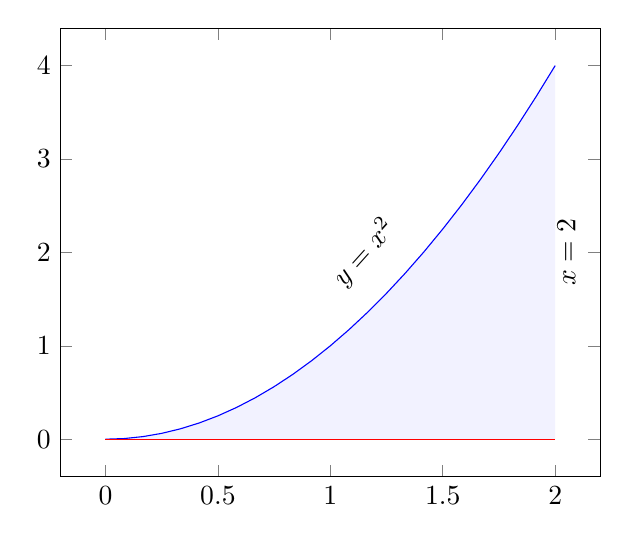
\begin{tikzpicture}
	\begin{axis}
	\addplot[name path=f,domain=0:2,blue] {x^2};
	\path[name path=axis] (axis cs:0,0) -- (axis cs:2,0);
	\draw [red] (axis cs:0,0) -- (axis cs:2,0);
	\addplot [
        thick,
        color=blue,
        fill=blue, 
        fill opacity=0.05
	]
    fill between[
        of=f and axis,
        soft clip={domain=0:2},
    ];
    \node [rotate=48] at (axis cs:  1.15,  2) {$y=x^2$};
    \node [rotate=90] at (axis cs:  2.05,  2) {$x=2$};
	\end{axis}
\end{tikzpicture}
  \caption{$D=\left\{(x,y) \ | \ 0 \leq x \leq 2 \ , \ 0 \leq y \leq x^2\right\}$} \label{fig:9.1}
\end{figure}

\newpage
Låt $f(x,y) = xy^2$ \newline
Vad blir volymen mellan ytan $z = xy^2$ och $xy$-planet ovanför D?

\begin{figure}[ht] 
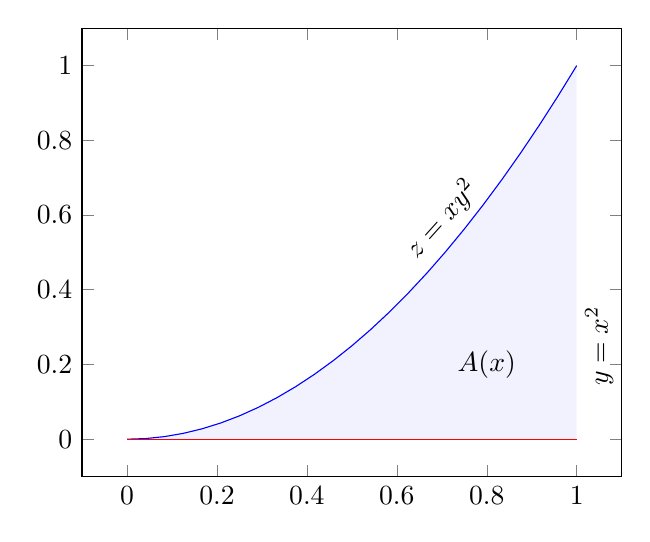
\begin{tikzpicture}
	\begin{axis}
	\addplot[name path=f,domain=0:1,blue] {x^2};
    \path[name path=axis] (axis cs:0,0) -- (axis cs:1,0);
	\draw [red] (axis cs:0,0) -- (axis cs:1,0);
    \addplot [
        thick,
        color=blue,
        fill=blue, 
        fill opacity=0.05
    ]
    fill between[
        of=f and axis,
        soft clip={domain=0:1},
    ];
    \node [rotate=48] at (axis cs:  .7,  .59) {$z=xy^2$};
    \node [rotate=90] at (axis cs:  1.05,  .25) {$y=x^2$};
    \node at (axis cs: 0.8,0.2) {$A(x)$};
	\end{axis}
\end{tikzpicture}
  \caption{2D representation av en skiva} \label{fig:9.2}
\end{figure}

$$
	A(x) = \int_0^{x^2}xy^2 \,\mathrm{d}y = x \int_0^{x^2} y^2 \,\mathrm{d}y = x\left[\frac{y^3}{3}\right]^{x^2}_0 = x \frac{x^6}{3} = \frac{x^7}{3}
$$

$$
	\text{Volymen }V = \int_0^2 A(x)\,\mathrm{d}x = \int_0^2 \frac{x^7}{3} \,\mathrm{d}x = \left[\frac{x^8}{24}\right]_0^2 = \frac{256}{24} = \frac{32}{3}
$$
Vi skriver dubbelintegralen av $xy$ över D
$$
	V = \int_0^2\left(\int_0^{x^2} xy^2 \,\mathrm{d}y \right)\,\mathrm{d}x = \iint_D xy^2 \,\mathrm{d}x\,\mathrm{d}y = \int_0^4 \left( \int_{\sqrt{2}}^2 xy^2 \,\mathrm{d}x \right) \,\mathrm{d}y
$$

\subsubsection{Skiva i \texorpdfstring{$y$}{y}-led}

$$
	A(y) = \int_{\sqrt{y}}^2 xy^2 \,\mathrm{d}x = y^2 \int_{\sqrt{y}}^2 x \,\mathrm{d}x = y^2 \left[\frac{x^2}{2}\right]_{\sqrt{2}}^2 = y^2\left(2- \frac{y}{2}\right) = 2y^2 - \frac{y^3}{2}
$$
$$
	V = \int_0^4 A(y) \,\mathrm{d}y = \int_0^4 \left(2- \frac{y}{2}\right)\,\mathrm{d}y = \left[\frac{2y^3}{3} - \frac{y^4}{8}\right]_0^4 = \frac{128}{3} - \frac{258}{8} = \frac{32}{3}
$$
Samma svar såklart!

\newpage
\subsection{Översikt, definition av dubbelintegraler}
Att integrera en variable i taget kallas \underline{upprepade enkelintegraler}
\subsubsection{Steg 1}

\begin{figure}[ht] 
\begin{tikzpicture}
   \tkzInit[xmax=5,ymax=5,xmin=-1,ymin=-1]
   \tkzAxeXY
   \draw (1,1) rectangle (5,4);
   \draw[blue] (1,1) rectangle (2,3);
   \draw[red] (2,1) rectangle (3.5,2);
   \node[above] at (5,4) {$\triangle$};
\end{tikzpicture}
  \caption{Visar på en yta med mindre ytor i} \label{fig:9.3}
\end{figure}

$\triangle =$ axelparallell rektangel \newline
Dela in $\triangle$ i små rektanglar $\triangle_1,\ldots,\triangle_n$ \newline

En trappfunktion $\phi$ på $\triangle_1,\ldots,\triangle_n$ är konstant på varje $\triangle_j \,:\, \phi(x,y) = C_j$ på $\triangle_j$. Då kan dubbelintegralen av $\phi$ över $\triangle$ definieras som volymen (med tecken)
$$
	\iint_\triangle \phi(x,y) \,\mathrm{d}x\,\mathrm{d}y = I(\phi) = C_1A(\triangle_1) + \ldots + C_nA(\triangle_n)
$$

\newpage
\subsubsection{Steg 2} \label{sec:Steg 2}
Om $\phi_1 \leq f \leq \phi_2$ på $\triangle$, $\phi_1, \, \phi_2$ trappfunktioner, så kallas $I(\phi_1)$ en undersumma till $f$ på $\triangle$ och $I(\phi_2)$ en översumma. 
$f$ kallas \underline{integrerbar} över $\triangle$ om $\forall \epsilon > 0 \, \exists$ sådana $\phi_1, \, \phi_2$ med $I(\phi_2) - I(\phi_1) < \epsilon$.
Man kan bevisa att då finns ett unikt tal $k$ så att $I(\phi_1) \leq k \leq I(\phi_2) \forall$ sådana $\phi_1, \, \phi_2, \, k$ kallas dubbelintegralen av $f$ över $\triangle$, skrivs
$$
	k = \iint_\triangle f(x,y) \,\mathrm{d}x\,\mathrm{d}y
$$
Kort sammanfattning:
\begin{framed}
	Man visar att $f$ kontinuerlig på $\triangle \Rightarrow f$ integrerbar över $\triangle$
\end{framed}

\subsubsection{Steg 3}
$D$ är en godtycklig mängd, $D \subset \triangle$ \newline
$$
	\text{Sätt } f_D = 
	\begin{cases}
		f & \quad \text{på } D \\
		0 & \quad \text{utanför } D \\
  	\end{cases}
  	\quad \text{, normalt sett ej kontinuerlig på randen av } D
$$
$f$ är integrerbar över $D$ om $f_D$ är integrerbar över $\triangle$ och då definieras

$$
	\iint_D f(x,y) \,\mathrm{d}x\,\mathrm{d}y = \underbrace{\iint_\triangle f_\mathrm{d}(x,y) \,\mathrm{d}x\,\mathrm{d}y}_{\text{definierat i \vref{sec:Steg 2}}}
$$

Man visar att $\iint_D f(x,y) \,\mathrm{d}x\,\mathrm{d}y \, \exists$ om $D$ begränsad, $f$ beror på $D$ $\Big( \abs{f(x,y)} \leq M \text{ på } D \Big)$ och $f$ kontinuerlig utom möjligen på en \underline{nollmängd};
en mängd $N$ som $\forall \epsilon > 0$ kan täckas över med rektanglar med total area $< \epsilon$. T.ex. kan $N$ vara en vanlig kurva (som $D$:s rand). \newline

Vanliga räknelagar gäller, t.ex. 

$$
	\iint_D \Big(f(x,y)+g(x,y)\Big) \,\mathrm{d}x\,\mathrm{d}y = \iint_D f(x,y) \,\mathrm{d}x\,\mathrm{d}y + \iint_D g(x,y) \,\mathrm{d}x\,\mathrm{d}y
$$

\newpage
\subsubsection{Exempel}
Beräkna $I = \iint_D x\sin{xy} \,\mathrm{d}x\,\mathrm{d}y$   då $D: 
\begin{cases}
	0 \leq x \leq \frac{\pi}{2} \\
	0 \leq y \leq 1 \\
\end{cases}$

Enklast att börja med att integrera över $y$

\begin{align*}
	I &= \int_0^{\frac{\pi}{2}} \left(\int_{y=0}^{y=1} x\sin{xy} \,\mathrm{d}y \right) \,\mathrm{d}x = \int_0^{\frac{\pi}{2}} \Bigg[ -\cos{xy} \Bigg]_{y=0}^{y=1} \,\mathrm{d}x = \\
	  &= \int_0^{\frac{\pi}{2}} \Bigg( -\cos{x} + 1 \Bigg) \,\mathrm{d}x = \Bigg[ -\sin{x} + x \Bigg]_0^{\frac{\pi}{2}} = -1 + \frac{\pi}{2}
\end{align*}

\subsubsection{Exempel}
Beräkna $I = \int_0^1 \left( \int_{x^2}^1 xe^{y^2} \,\mathrm{d}y \right) \,\mathrm{d}x$    $\int e^{y^2} \,\mathrm{d}y = ???$ Enklare att börja med $x$

\begin{figure}[ht] 
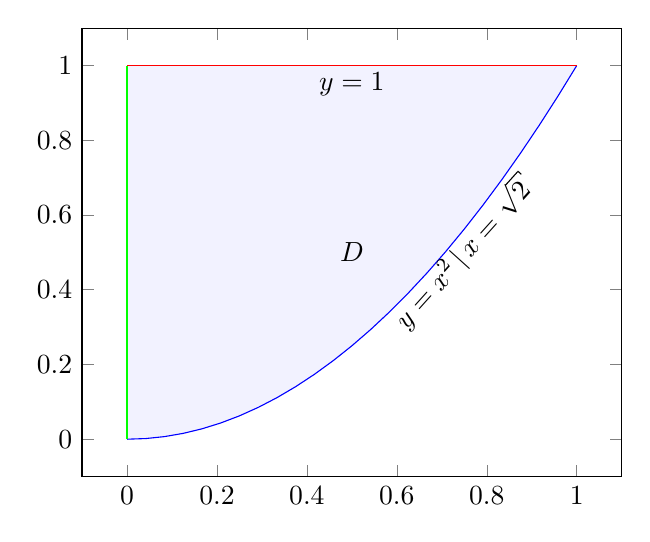
\begin{tikzpicture}
	\begin{axis}
	\addplot[name path=f,domain=0:1,blue] {x^2};
    \path[name path=axis] (axis cs:0,1) -- (axis cs:1,1);
	\draw [red] (axis cs:0,1) -- (axis cs:1,1);
	\draw [green] (axis cs:0,0) -- (axis cs:0,1);
    \addplot [
        thick,
        color=blue,
        fill=blue, 
        fill opacity=0.05
    ]
    fill between[
        of=axis and f,
        soft clip={domain=0:1},
    ];
    \node [rotate=48] at (axis cs:  .75,  .5) {$y=x^2 \, | \, x=\sqrt{2}$};
    \node at (axis cs:  .5, .95) {$y=1$};
    \node at (axis cs: 0.5,0.5) {$D$};
	\end{axis}
\end{tikzpicture}
  \caption{$D={(x,y) \, | \, 0 \leq y \leq 1 \, 0 \leq x \leq \sqrt{y}}$} \label{fig:9.4}
\end{figure}

\begin{align*}
	\Rightarrow I &= \int_0^1 \left( \int_0^{\sqrt{y}} xe^{y^2} \,\mathrm{d}x \right) \,\mathrm{d}y = \int_0^1 e^{y^2} \left[\frac{x^2}{2}\right]_0^{\sqrt{2}} \,\mathrm{d}y = \\
	              &= \int_0^1 e^{y^2} \frac{y}{2} \,\mathrm{d}y = \frac{1}{2} \int_0^1 ye^{y^2} \,\mathrm{d}y = \frac{1}{4} \Bigg[ e^{y^2} \Bigg]_0^1 = \frac{e-1}{4}
\end{align*}

\newpage
\subsection{Definition} 
\underline{Arean} av en mängd $D$ i $xy$-planet är Arean$(D) = \iint_D \,\mathrm{d}x\,\mathrm{d}y$ \label{subsec:Area}

\subsubsection{Exempel}

\begin{align*}
	D: &
	\begin{cases}
	a \leq x \leq b \\
	f(x) \leq y \leq g(x) \\
	\end{cases}
\text{   , ger Area}(D) = \iint_D \,\mathrm{d}x\,\mathrm{d}y = \\
&= \int_a^b \left( \int_{f(x)}^{g(x)} \,\mathrm{d}y \right) \,\mathrm{d}x = \int_a^b \Bigg[ y \Bigg]_{f(x)}^{g(x)} \,\mathrm{d}x = \\
&= \underbrace{\int_a^b \Big(g(x) - f(x) \Big) \,\mathrm{d}x}_{\text{bekant från envarre}}
\end{align*}







\newpage
\section{Föreläsning X}
\subsection{Variabelbyte i dubbelintegraler - Sats}
Om $D$ i $xy$-planet avbildas \underline{bijektivt} på $E$ i $uv$-planet (till varje punkt $(x,y) \in D$ hör en punkt $(u,v) \in E$ och omvänt) med \(\frac{\mathrm{d}(x,y)}{\mathrm{d}(u,v)} = 
\begin{vmatrix}
	x'_u & x'_v \\
	y'_u & y'_v
\end{vmatrix} \neq 0\)
så är $\iint_D f(x,y) \,\mathrm{d}x\,\mathrm{d}y = \iint_E f\Big( x(u,v),y(u,v) \Big)\abs{\frac{\mathrm{d}(x,y)}{\mathrm{d}(u,v)}}\,\mathrm{d}u\,\mathrm{d}v$
\subsubsection{Bevisidé}
Approximera trappfunktionen $\phi$ \newline
För att integralens värde inte ska ändras måste vi multiplicera med 
$$
	\frac{1}{
	\begin{vmatrix}
		\frac{\mathrm{d}(u,v)}{\mathrm{d}(x,y)}
	\end{vmatrix}}
	= \frac{1}{
	\begin{vmatrix}
		u'_x & u'_y \\
		v'_x & v'_y
	\end{vmatrix}}
	= 
	\begin{vmatrix}
		x'_u & x'_v \\
		y'_u & y'_v
	\end{vmatrix} 
	= \frac{\mathrm{d}(x,y)}{\mathrm{d}(u,v)}
$$

Jämför med envarre: $\mathrm{d}x = \frac{\mathrm{d}x}{\mathrm{d}t}\,\mathrm{d}t$ \newline

Belopp på determinant i flervarre för att vi alltid sätter gränser från undre till övre värde

\subsubsection{Exempel}

$$I = \iint_D \frac{\mathrm{d}x\,\mathrm{d}y}{5+x^2+y^2} \; , \; D=\Big\{(x,y) \, | \, x^2+y^2 \leq 3 \, x \leq 0 \, y \geq 0\Big\}$$

$$\text{Byt till polära koordinater: } \left\{
\begin{array}{rcl}
	x = \rho\cos{\varphi} \\
	y = \rho\sin{\varphi}
\end{array}\right.
\Rightarrow D\text{ övergår i } E$$

$$E: 
\begin{cases}
	0 \leq \rho \leq \sqrt{3} \\
	\frac{\pi}{2} \leq \varphi \leq \pi
\end{cases} 
\frac{\,\mathrm{d}x\,\mathrm{d}y}{\,\mathrm{d}\rho\,\mathrm{d}\varphi} = \text{se \vref{Rho}} = \rho $$

\begin{align*}
\Rightarrow I &= \iint_E \frac{1}{5+\rho^2}
\begin{vmatrix}
	\frac{\,\mathrm{d}x\,\mathrm{d}y}{\,\mathrm{d}\rho\,\mathrm{d}\varphi}
\end{vmatrix}
\,\mathrm{d}\rho\,\mathrm{d}\varphi = \int_\frac{\pi}{2}^\pi \left( \int_0^{\sqrt{3}} \frac{\rho}{5+\rho^2} \,\mathrm{d}\rho \right)\,\mathrm{d}\varphi = \\
&= \int_\frac{\pi}{2}^\pi \left[ \frac{1}{2} \ln{5+\rho^2} \right]_0^{\sqrt{3}} \,\mathrm{d}\varphi = \int_\frac{\pi}{2}^\pi \left( \frac{1}{2} \ln{8} - \frac{1}{2} \ln{5} \right) \,\mathrm{d}\varphi = \\
&= \frac{1}{2} \ln{\frac{8}{5}} \int_\frac{\pi}{2}^\pi \,\mathrm{d}\varphi = \frac{1}{2}\ln{\frac{8}{5}} \Big[\rho\Big]_\frac{\pi}{2}^\pi = \svar{\frac{\pi}{4}\ln{\frac{8}{5}}}
\end{align*}

\newpage
\subsubsection{På en elipsskiva}

$$\left(\frac{x-x_o}{a}\right)^2 + \left(\frac{y-y_o}{b}\right)^2 \leq 1$$

\begin{figure}[ht]
\usetikzlibrary{patterns}
\begin{tikzpicture}
   \tkzInit[xmax=5,ymax=4,xmin=-1,ymin=-1]
   \tkzAxeXY
   \draw[pattern=north west lines, pattern color=blue] (1.5,1.5) ellipse (2 and 1);
  \end{tikzpicture}
  \caption{Funktion i $xy$-planet} \label{fig:10.1}
\end{figure}

$$
	\text{Variabelbytet }
	\begin{cases}
		u = \frac{x-x_o}{a} \\
		v = \frac{y-y_o}{b}
	\end{cases}
	\text{, ger } u^2+y^2 \leq 1
	\text{ och } \frac{\,\mathrm{d}(x,y)}{\,\mathrm{d}(u,v)} = \frac{1}{
	\begin{pmatrix}
		u'_x & u'_y \\
		v'_x & v'_y
	\end{pmatrix}} = \frac{1}{
	\begin{pmatrix}
		\frac{1}{a} & 0 \\
		0 & \frac{1}{b}
	\end{pmatrix}} = \frac{1}{\frac{1}{ab}} = ab
$$

\begin{figure}[ht]
\usetikzlibrary{patterns}
\begin{tikzpicture}
   \tkzInit[xmax=2,ymax=2,xmin=-2,ymin=-2]
   \tkzAxeX[label=$u$, above=10pt]
   \tkzAxeY[label=$v$, right=10pt]
   \draw[pattern=north west lines, pattern color=red] (0,0) circle (1);
\end{tikzpicture}
  \caption{Avbildat i $uv$-planet} \label{fig:10.2}
\end{figure}

$\,\mathrm{d}x\,\mathrm{d}y$ byts mot $ab\,\mathrm{d}u\,\mathrm{d}v$, sedan kan $u,v$ bytas mot polära $\frac{\,\mathrm{d}(u,v)}{\,\mathrm{d}(\rho,\varphi)} = \rho$

\newpage
\subsection{Trippelintegraler}

$$\iiint_D f(x,y,z) \,\mathrm{d}x\,\mathrm{d}y\,\mathrm{d}z$$

definieras också med över- och undersummor. Ingen rent geometrisk tolkning i 3D ty behövs $4$ axlar för $x,y,z$ och $f$. 
Fysikaliska tolkningar är att om $f(x,y,z)$ är en densitet/täthet (mass-,laddnigs-,...) så ger integralen det totala värdet på storheten (massa,laddning,...). \newline

\underline{Volymen} av $D$ \underline{definieras} som
$$\iiint_D \,\mathrm{d}x\,\mathrm{d}y\,\mathrm{d}z \text{  (som area i 2D, se \vref{subsec:Area})}$$

Trippelintegraler och multipelintegraler
$$\idotsint_D f(x_1,\ldots,x_n) \,\mathrm{d}x_1,\ldots,\,\mathrm{d}x_n \: ,\, n \geq 4$$
kan beräknas med upprepade enkelintegraler

\subsubsection{Exempel} \label{subsec:intordn}

Beräkna $I = \iiint_D z \,\mathrm{d}x\,\mathrm{d}y\,\mathrm{d}z$ då $D$ ges av 
$\begin{cases}
	0 \leq x \leq 1 \\
	x \leq y \leq 1 \\
	0 \leq z \leq (y-x)^2
\end{cases}$

\begin{align*}
	I &= \int_0^1 \left(\int_x^1 \left( \int_0^{(y-x)^2} z\,\mathrm{d}z\right)\,\mathrm{d}y\right)\,\mathrm{d}x = 
	\int_0^1 \left(\int_x^1 \left[ \frac{z^2}{2} \right]_0^{(y-x)^2}\,\mathrm{d}y\right)\,\mathrm{d}x = \\
	&= \int_0^1 \left(\left[\frac{(y-x)^5}{10}\right]_x^1\right)\,\mathrm{d}x = 
	\int_0^1 \left(\frac{(1-x)^5}{10} - \frac{(x-x)^5}{10}\right)\,\mathrm{d}x = \\
	&= \left[-\frac{(1-x)^6}{60}\right]_0^1 =
	0 - \left(-\frac{1}{60}\right) =
	\svar{\frac{1}{60}}
\end{align*}

\newpage
\subsection{Integrationsordningar}
Det finns $6$ olika integrationsordningar, ovan \vref{subsec:intordn} tog vi $z\rightarrow y\rightarrow x$.

Med $z$ först har vi kvar projektionen $D_{xy}$ av $D$

$$
z\rightarrow y\rightarrow x \text{ ger } (1)
\begin{cases}
&\left.\begin{array}{rcl}
0 \leq &x \leq 1 \\
x \leq &y \leq 1 \end{array}\right\}	D_{xy} \\
&0 \leq z \leq (y-x)^2
\end{cases}
$$


$$ \label{eq:10.1}
z\rightarrow x\rightarrow y \text{ ger } (2)
\begin{cases} 
&\left.\begin{array}{rcl}
0 \leq &y \leq 1 \\
0 \leq &x \leq y \end{array}\right\}	D_{xy} \\
&0 \leq z \leq (y-x)^2
\end{cases}
$$


Med $y$ först har vi kvar projektionen $D_{xz}$ av $D$ \newline
$\begin{cases}
z = (y-x)^2 \Rightarrow \sqrt{z} = \pm (y-x) \Rightarrow y = x+\sqrt{z} \\
z = (1-x)^2 \Rightarrow x = 1 - \sqrt{z}
\end{cases}$


$$
y\rightarrow z\rightarrow x \text{ ger } (3)
\begin{cases}
&\left.\begin{array}{rcl}
0 \leq &x \leq 1 \\
x \leq &z \leq (1-x)^2 \end{array}\right\} D_{xz} \\
&x+\sqrt{z} \leq y \leq 1
\end{cases}
$$


$$
y\rightarrow x\rightarrow z \text{ ger } (4)
\begin{cases}
&\left.\begin{array}{rcl}
0 \leq &z \leq 1 \\
0 \leq &x \leq 1-\sqrt{z} \end{array}\right\} D_{xz} \\
&x+\sqrt{z} \leq y \leq 1
\end{cases}
$$


Med $x$ först har vi kvar projektionen $D_{yz}$ av $D$


$$ \label{eq:10.2}
x\rightarrow z\rightarrow y \text{ ger } (5)
\begin{cases}
&\left.\begin{array}{rcl}
0 \leq &y \leq 1 \\
x \leq &z \leq y^2 \end{array}\right\}	D_{yz} \\
&0 \leq x \leq y - \sqrt{z}
\end{cases}
$$


$$
x\rightarrow y\rightarrow z \text{ ger } (6)
\begin{cases}
&\left.\begin{array}{rcl}
0 \leq &z \leq 1 \\
\sqrt{z} \leq &y \leq 1 \end{array}\right\}	D_{yz} \\
&0 \leq x \leq y - \sqrt{z}
\end{cases}
$$

\newpage
\begin{figure}[ht]
\resizebox{4cm}{4cm}{
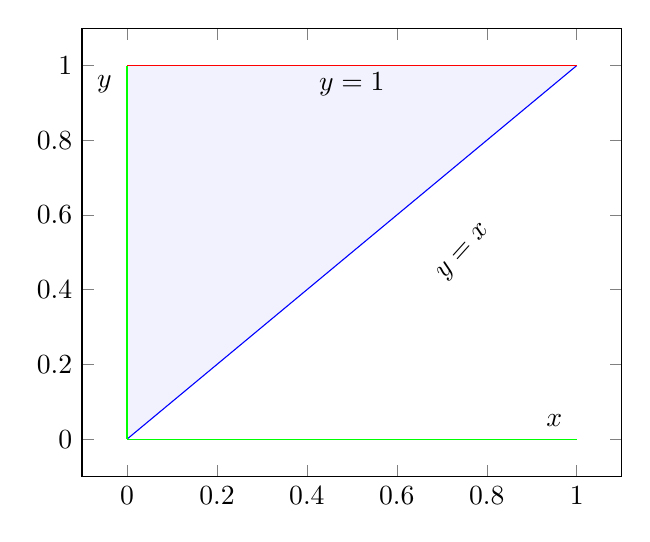
\begin{tikzpicture}
	\begin{axis}
	\addplot[name path=f,domain=0:1,blue] {x};
    \path[name path=axis] (axis cs:0,1) -- (axis cs:1,1);
	\draw [red] (axis cs:0,1) -- (axis cs:1,1);
	\draw [green] (axis cs:0,0) -> (axis cs:0,1);
	\draw [green] (axis cs:0,0) -> (axis cs:1,0);
    \addplot [
        thick,
        color=blue,
        fill=blue, 
        fill opacity=0.05
    ]
    fill between[
        of=axis and f,
        soft clip={domain=0:1},
    ];
    \node [rotate=48] at (axis cs:  .75,  .5) {$y=x$};
    \node at (axis cs: .5,.95) {$y=1$};
    \node at (axis cs: -.05,.95) {$y$};
    \node at (axis cs: .95,.05) {$x$};
	\end{axis}
\end{tikzpicture}}
  \caption{$D_{xy}$} \label{fig:10.3}
\end{figure}

\begin{figure}[ht]
\resizebox{4cm}{4cm}{
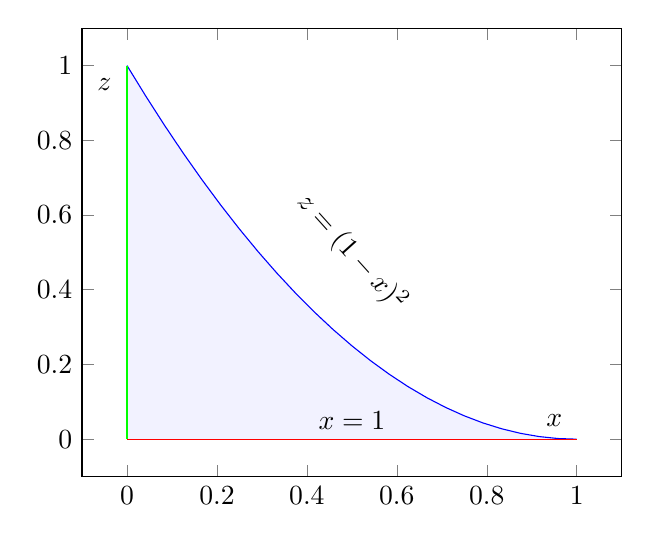
\begin{tikzpicture}
	\begin{axis}
	\addplot[name path=f,domain=0:1,blue] {(1-x)^2};
    \path[name path=axis] (axis cs:0,0) -- (axis cs:1,0);
	\draw [red] (axis cs:0,0) -- (axis cs:1,0);
	\draw [green] (axis cs:0,0) -> (axis cs:0,1);
    \addplot [
        thick,
        color=blue,
        fill=blue, 
        fill opacity=0.05
    ]
    fill between[
        of=axis and f,
        soft clip={domain=0:1},
    ];
    \node [rotate=-48] at (axis cs:  .5,  .5) {$z=(1-x)^2$};
    \node at (axis cs: .5,.05) {$x=1$};
    \node at (axis cs: -.05,.95) {$z$};
    \node at (axis cs: .95,.05) {$x$};
	\end{axis}
\end{tikzpicture}}
  \caption{$D_{xz}$} \label{fig:10.4}
\end{figure}

\begin{figure}[ht]
\resizebox{4cm}{4cm}{
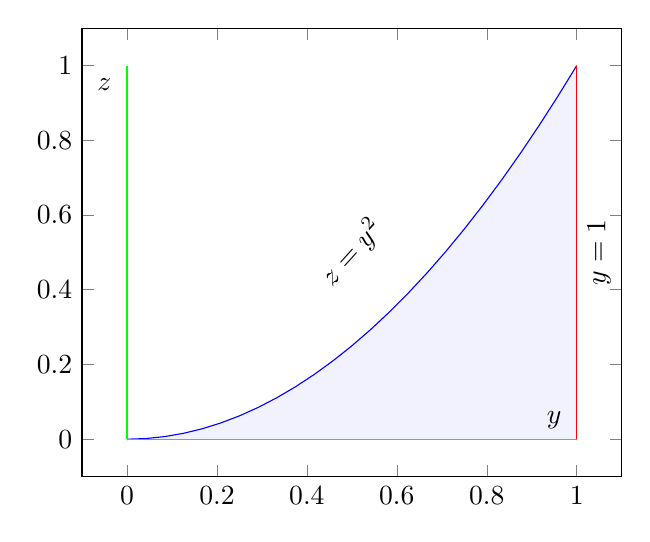
\begin{tikzpicture}
	\begin{axis}
	\addplot[name path=f,domain=0:1,blue] {x^2};
    \path[name path=axis] (axis cs:0,0) -- (axis cs:1,0);
	\draw [red] (axis cs:1,0) -- (axis cs:1,1);
	\draw [green] (axis cs:0,0) -> (axis cs:0,1);
	\draw [green] (axis cs:0,0) -> (axis cs:1,0);
    \addplot [
        thick,
        color=blue,
        fill=blue, 
        fill opacity=0.05
    ]
    fill between[
        of=f and axis,
        soft clip={domain=0:1},
    ];
    \node [rotate=48] at (axis cs: .5,.5) {$z=y^2$};
    \node [rotate=90] at (axis cs: 1.05,.5) {$y=1$};
    \node at (axis cs: -.05,.95) {$z$};
    \node at (axis cs: .95,.05) {$y$};
	\end{axis}
\end{tikzpicture}}
  \caption{$D_{yz}$} \label{fig:10.5}
\end{figure}

\newpage
Test av \eqref{eq:10.2} 
\begin{align*}
	I &= \int_0^1 \int_0^{y^2} \int_0^{y-\sqrt{z}} z \,\mathrm{d}x\,\mathrm{d}\,\mathrm{d}z\,\mathrm{d}y =
	\int_0^1 \int_0^{y^2} z \Big[x\Big]_0^{y-\sqrt{z}} \,\mathrm{d}z\,\mathrm{d}y=
	\int_0^1 \int_0^{y^2} z(y-\sqrt{z}) \,\mathrm{d}z\,\mathrm{d}y = \\
	&= \int_0^1 \Big[ \frac{z^2y}{2} - \frac{2z^{\frac{5}{2}}}{5} \Big]_0^{y^2} \,\mathrm{d}y =
	\int_0^1 \Big( \frac{y^2}{2} - \frac{2y^5}{5} - \frac{0^2y}{2} - \frac{2*0^{\frac{5}{2}}}{5} \Big) \,\mathrm{d}y = \\
	&= \int_0^1 \frac{y^5}{10} \,\mathrm{d}y = 
	\Big[ \frac{y^6}{60} \Big] = \svar{\frac{1}{60}}
\end{align*}

Man kan också tänka att $D$ skivas upp. T.ex. för \underline{fixt} $y$ har vi skivan i figur \vref{fig:10.4}

$$
	\text{Ger } I = \int_0^1 \Big( \iint_{\hat{D}_{xz}} \,\mathrm{d}x\,\mathrm{d}z \Big)\,\mathrm{d}y
$$

$$
	\hat{D}_{xz} : 
	\begin{cases}
		0 \leq x \leq y \\
		0 \leq z \leq (y-x)^2
	\end{cases}
	\text{ ger } \eqref{eq:10.1}
$$

$$
	\hat{D}_{xz} : 
	\begin{cases}
		0 \leq z \leq y^2 \\
		0 \leq x \leq y-\sqrt{z}
	\end{cases}
	\text{ ger } \eqref{eq:10.2}
$$




\newpage
\section{Föreläsning XI}

Kommer snart!









\newpage
\fancyhf{}
\rhead{\textit{Adnan Avdagic}}
\lhead{Appendix}
\pagenumbering{gobble}
\section{Appendix}
\begin{appendix}
	\listoffigures
	\listoftables
\end{appendix}
\end{document}